\documentclass{ctexart}

% https://tex.stackexchange.com/questions/279/how-do-i-ensure-that-figures-appear-in-the-section-theyre-associated-with
\usepackage[section]{placeins}

\usepackage{geometry}
\geometry{
    a4paper,
    left=1.91cm,
    right=1.91cm,
    top=2.54cm,
    bottom=2.54cm
}

\usepackage{hyperref}

\usepackage{graphicx}

\usepackage{subcaption}

\pagestyle{plain}

\ctexset {
    section = {
        format = \Large\bfseries,
    }
}

\usepackage{listings}

% https://www.overleaf.com/learn/latex/Code_Highlighting_with_minted
% https://www.overleaf.com/learn/latex/Questions/Which_programming_languages_does_the_minted_package_support%3F https://pygments.org/languages/
\usepackage{minted}

\title{GAMES104: PA2}

\begin{document}
    
    \maketitle
    
    \section{基础:颜色分级} \label{section:basic1}
    在实现Color Grading功能的过程中,遇到最为棘手的问题就是输出效果异常,尽管参考了多位同学的代码,使用RenderDoc初步调试,还是没有找到原因。
    虽然最终在计算机图形学与混合现实在线平台论坛中找到这篇帖子\href{https://games-cn.org/forums/topic/guanyuzuoye2shuchuwenti/}{“关于作业2输出问题”},在games104/homework02-rendering分支下同样的代码输出正常,Commit on Oct 23, 2023 92a171e5aeb9e752bbf74afbbf72661a247b722e 出现输出效果异常的原因还需要进一步研究。此外帖子\href{https://games-cn.org/forums/topic/zuoye2-pa02-youyongdexinxiheji/}{“作业2 PA02 有用的信息合集”}中分享了教程\href{https://defold.com/tutorials/grading/}{“Grading tutorial ”}。
    
    这篇帖子\href{https://games-cn.org/forums/topic/guanyuzuoyeerqulutdewenti/}{“关于作业二,取LUT的问题”}中提到的教程\href{https://games-cn.org/forums/topic/guanyuzuoyeerqulutdewenti/}{“3D Game Shaders For Beginners”}对于LUT实现细节讲解的比较深入,但是在完成作业时,仍然需要结合引擎实际逻辑来完成代码编写。首先参考\href{https://en.wikipedia.org/wiki/OpenGL_Shading_Language}{维基百科}对于GLSL版本说明可以找到文档\href{https://registry.khronos.org/OpenGL/specs/es/3.1/GLSL_ES_Specification_3.10.withchanges.pdf}{The OpenGL ES Shading Language}    
    \begin{minted}{GLSL}
#version 310 es
    \end{minted}
    \verb|textureSize()|函数返回\textbf{LUT PNG Texture}图片像素大小,仓库预先提供的LUT图片包含$ 256\times16 $和$ 1024\times32 $这两种规格。\textbf{Color Grading}管线需要完成的颜色映射,输入的颜色数值 $ \in [0,1] $, 输出的颜色采样坐标数值$ \in [0,1] $,由于贴图是按像素离散存储,从输入颜色到输出采样需要根据贴图分布计算映射关系。为了实现自适应贴图映射,首先获取贴图大小,\textbf{textureSize}函数返回值为贴图分辨率的像素值,
    \begin{minted}{GLSL}
highp ivec2 lut_tex_size = textureSize(color_grading_lut_texture_sampler, 0);
    \end{minted}
    通过贴图大小\verb|lut_tex_size|计算贴图包含的像素数量\verb|lut_tex_pixel_count|,之后通过预设的贴图像素总数和单通道像素数的对应关系,获得单通道像素数\verb|lut_3d_pixel_size|
    \begin{minted}{GLSL}
highp int lut_tex_pixel_count = lut_tex_size.x * lut_tex_size.y;
highp float lut_3d_pixel_size;    
switch (lut_tex_pixel_count) {
    case 4069:
        lut_3d_pixel_size = 16.0;
        break;
    case 32768:
        lut_3d_pixel_size = 32.0;
        break;
    case 262144:
        lut_3d_pixel_size = 64.0;
        break;
}
    \end{minted}    
    通过\verb|lut_tex_size|和\verb|lut_3d_pixel_size|可以计算贴图中\textbf{Block}的分布$ 16\times1 $,$ 32\times1 $或者$ 8\times8 $。
    \begin{minted}{GLSL}
highp float cube_2d_pixel_size_x = float(lut_tex_size.x);
highp float cube_2d_pixel_size_y = float(lut_tex_size.y);
    \end{minted}
    \begin{minted}{GLSL}
highp float cube_2d_block_count_x = cube_2d_pixel_size_x / lut_3d_pixel_size;
highp float cube_2d_block_count_y = cube_2d_pixel_size_y / lut_3d_pixel_size;
    \end{minted}
    至此完成贴图排布的解析。由于\textbf{Color Grading}管线采用的是\textbf{Linear}采样器,所以理论上只需要在蓝色通道上做插值采样,采样的思路变成找到输入蓝色通道对应的LUT贴图的两个\textbf{Block},将这两个采样结果按照比例插值得到输出采样值。将输入颜色向贴图像素空间映射时,以像素分辨率为$ 512\times512 $的\textbf{Cube Grid 2D}贴图为例,当\verb|in_color.b|的值为0时,对应最左上角的\textbf{Block 00},当\verb|in_color.b|的值为1时,对应最右下角的\textbf{Block 15},代码中\verb|lut_3d_uniform_size|目的是为了从1开始的像素值映射到从0开始。
    \begin{minted}{GLSL}
highp float lut_3d_uniform_size = lut_3d_pixel_size - 1.0;
    \end{minted}
    \begin{minted}{GLSL}
highp float lut_3d_sample_pixel_z = lut_3d_uniform_size * color.b;
    \end{minted}
    以蓝色通道向下取整这个\textbf{Block}为例,分别计算\textbf{Block}视角下的偏移量。当贴图\textbf{Block}分布为$ 16\times1 $或$ 32\times1 $条带时,\verb|cube_z0_2d_block_sample_y|会始终为0,这与竖向分布个数为1相一致。当贴图\textbf{Block}分布为$ 8\times8 $格网时,当\verb|in_color.b|的值为1时,\verb|cube_z0_2d_block_sample_y|和\verb|cube_z0_2d_block_sample_x|均为7,对应从0开始的索引值。
    \begin{minted}{GLSL}
highp float lut_3d_sample_pixel_z0 = floor(lut_3d_sample_pixel_z);
highp float cube_z0_2d_block_sample_y = floor(lut_3d_sample_pixel_z0 / cube_2d_block_count_x);
highp float cube_z0_2d_block_sample_x = lut_3d_sample_pixel_z0 
- cube_z0_2d_block_sample_y * cube_2d_block_count_x;
    \end{minted}
    当获取到采样\textbf{Block}的位置后,计算x方向\textbf{Block}内部的偏移值\verb|lut_3d_sample_pixel_x|
    \begin{minted}{GLSL}
highp float lut_3d_sample_pixel_x = lut_3d_uniform_size * color.r;
    \end{minted}
    计算x方向\textbf{Block}最大的偏移值\verb|cube_2d_uniform_block_size_x|
    \begin{minted}{GLSL}
highp float cube_2d_uniform_block_size_x = lut_3d_pixel_size * (cube_2d_block_count_x - 1.0);
    \end{minted}
    计算x方向UV坐标归一化系数\verb|cube_2d_uniform_size_y|,
    \begin{minted}{GLSL}
highp float cube_2d_uniform_size_x = cube_2d_pixel_size_x - 1.0;
    \end{minted}
    求和、归一化得到采样UV坐标值。
    \begin{minted}{GLSL}
highp float cube_2d_sample_u_x_y_z0 
= (cube_z0_2d_block_sample_x / (cube_2d_block_count_x - 1.0) * cube_2d_uniform_block_size_x 
+ lut_3d_sample_pixel_x) / cube_2d_uniform_size_x;
    \end{minted}
    同样地在y方向上,计算\textbf{Block}内部的偏移值\verb|lut_3d_sample_pixel_y|
    \begin{minted}{GLSL}
highp float lut_3d_sample_pixel_y = lut_3d_uniform_size * color.g;
    \end{minted}
    计算\textbf{Block}最大的偏移值\verb|cube_2d_uniform_block_size_y|
    \begin{minted}{GLSL}
highp float cube_2d_uniform_block_size_y = lut_3d_pixel_size * (cube_2d_block_count_y - 1.0);
    \end{minted}
    计算y方向UV坐标归一化系数\verb|cube_2d_uniform_size_y|,
    \begin{minted}{GLSL}
highp float cube_2d_uniform_size_y = cube_2d_pixel_size_y - 1.0;
    \end{minted}
    需要注意地,当y方向\textbf{Block}数为1时,UV坐标中v的值和输入绿色通道的值相等。
    \begin{minted}{GLSL}
highp float cube_2d_sample_v_x_y_z0;
if (cube_2d_block_count_y == 1.0) {
    cube_2d_sample_v_x_y_z0 = color.g;
} else {
    cube_2d_sample_v_x_y_z0 
    = (cube_z0_2d_block_sample_y / (cube_2d_block_count_y - 1.0) * cube_2d_uniform_block_size_y 
    + lut_3d_sample_pixel_y) / cube_2d_uniform_size_y;
}
    \end{minted}
    构造UV坐标\verb|cube_2d_sample_uv_x_y_z1,|
\begin{minted}{GLSL}
highp vec2 cube_2d_sample_uv_x_y_z1 = vec2(cube_2d_sample_u_x_y_z1, cube_2d_sample_v_x_y_z1);
\end{minted}    
    通过函数\verb|texture|获得插值一侧的颜色\verb|cube_2d_sample_texture_x_y_z0|,
\begin{minted}{GLSL}
highp vec4 cube_2d_sample_texture_x_y_z0 = texture(
    color_grading_lut_texture_sampler,
    cube_2d_sample_uv_x_y_z0
);
\end{minted}     
    通过函数\verb|mix|将两侧的颜色插值后得到最后输出的颜色值。
\begin{minted}{GLSL}
highp vec4 cube_2d_sample_texture_x_y_z = mix(
    cube_2d_sample_texture_x_y_z0, 
    cube_2d_sample_texture_x_y_z1, 
    lut_3d_sample_fract_z
);
\end{minted}
    通过将一个3D LUT文件分别导出不同大小\textbf{Cube Strip 2D}和\textbf{Cube Grid 3D}来验证算法实现的正确性
    \begin{figure}[!htbp]
    	\centering
    	\begin{subfigure}{0.49\textwidth}
    		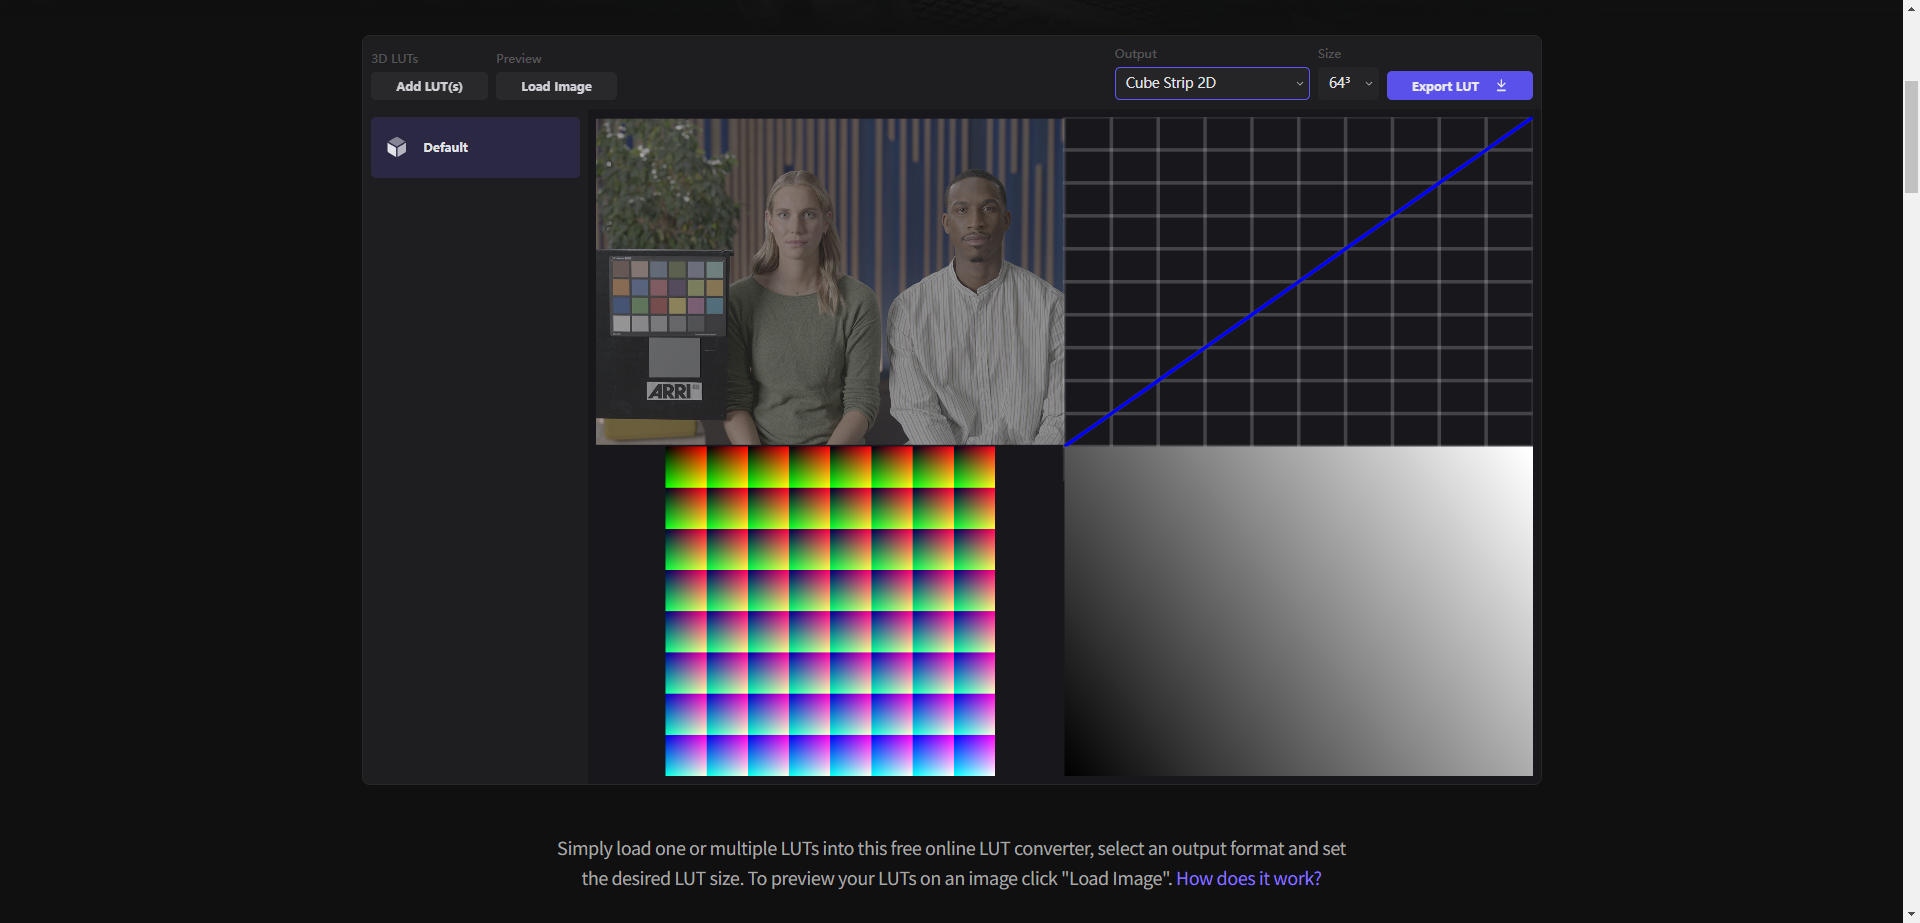
\includegraphics[width=\textwidth]{color.io_lut_converter_default.png}
    		\caption{caption\_for\_sub1}
    	\end{subfigure}
    	\begin{subfigure}{0.49\textwidth}
    		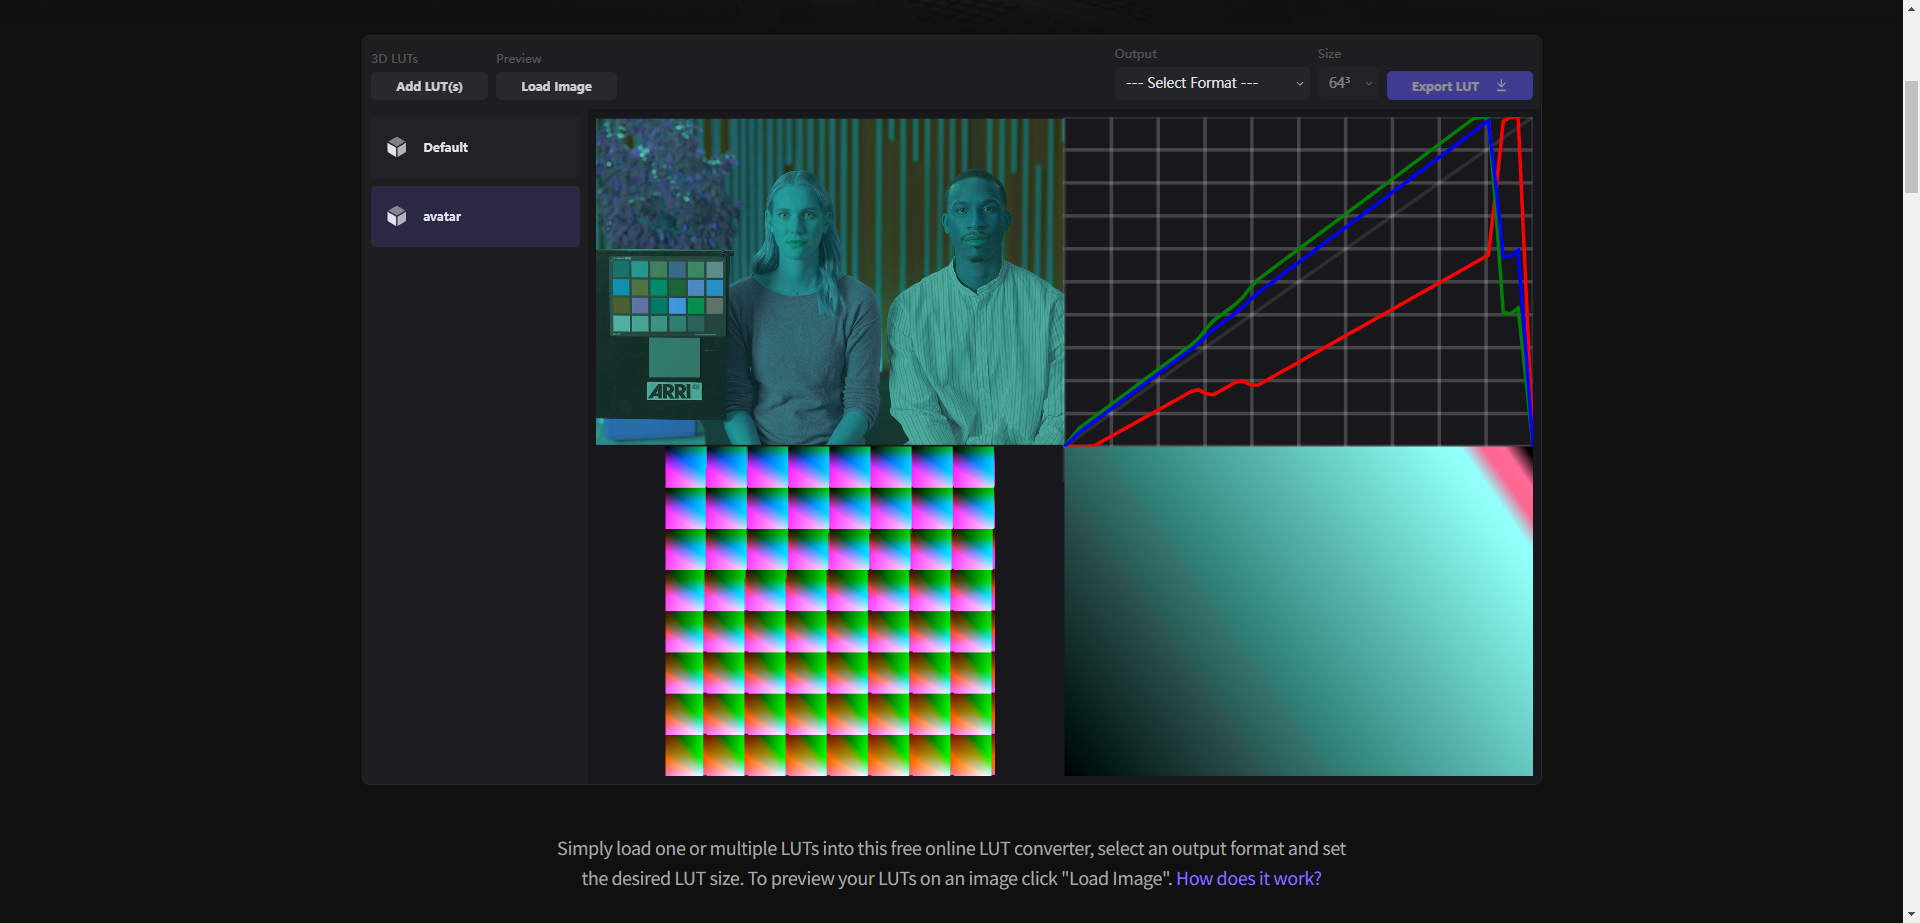
\includegraphics[width=\textwidth]{color.io_lut_converter_avatar.png}
    		\caption{caption\_for\_sub1}
    	\end{subfigure}      
    	\caption{3D LUT Avatar在线预览效果.png}
    \end{figure}
    通过观察天空的映射情况,Grid格式相比Strip效果会偏好。
    \begin{figure}[!htbp]
    	\centering
    	\begin{subfigure}{0.3\textwidth}
    		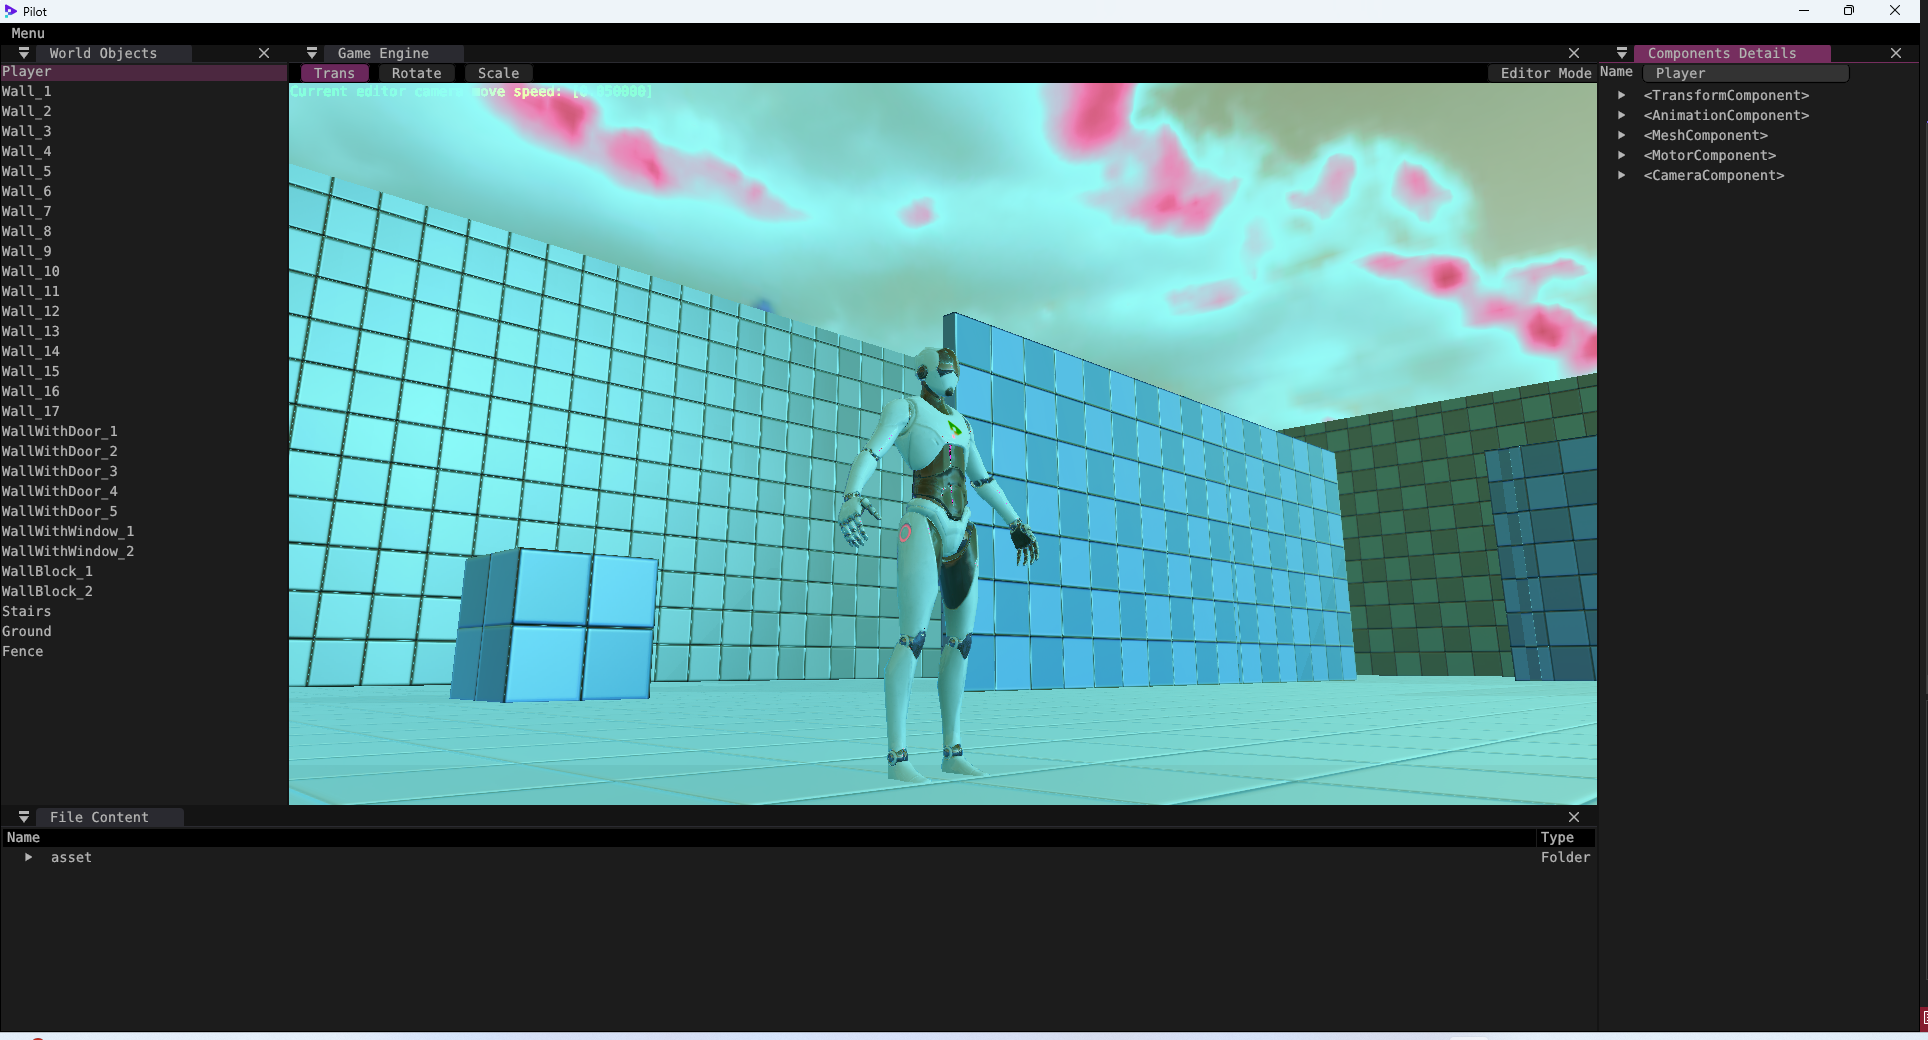
\includegraphics[width=\textwidth]{screen_shot_cube_strip_2d_16_avatar.png}
    		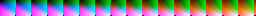
\includegraphics[width=\textwidth]{cube_strip_2d_16_avatar.png}
    		\caption{strip \& 16}
    	\end{subfigure}
    	\begin{subfigure}{0.3\textwidth}
    		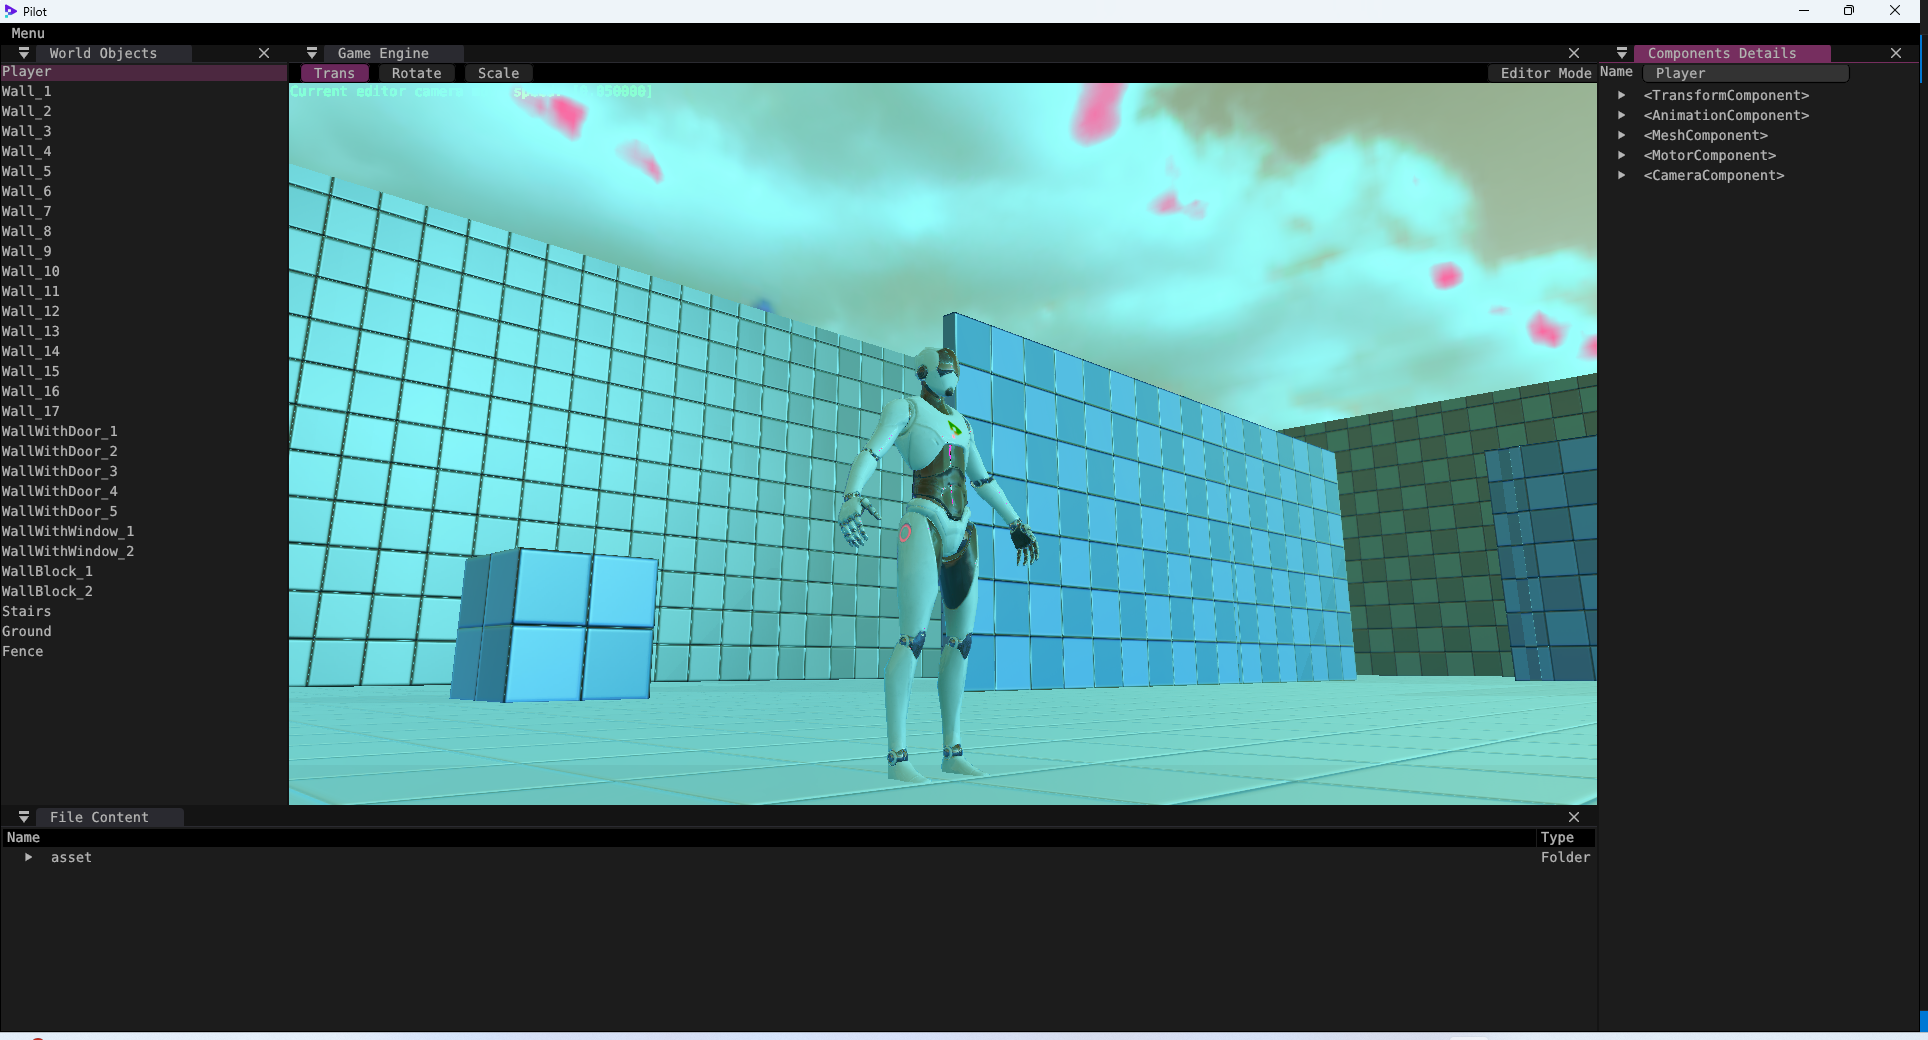
\includegraphics[width=\textwidth]{screen_shot_cube_strip_2d_32_avatar.png}
    		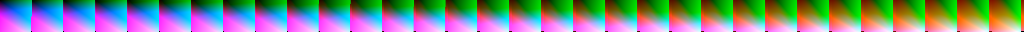
\includegraphics[width=\textwidth]{cube_strip_2d_32_avatar.png}
    		\caption{strip \& 32}
    	\end{subfigure}
    	\begin{subfigure}{0.3\textwidth}
    		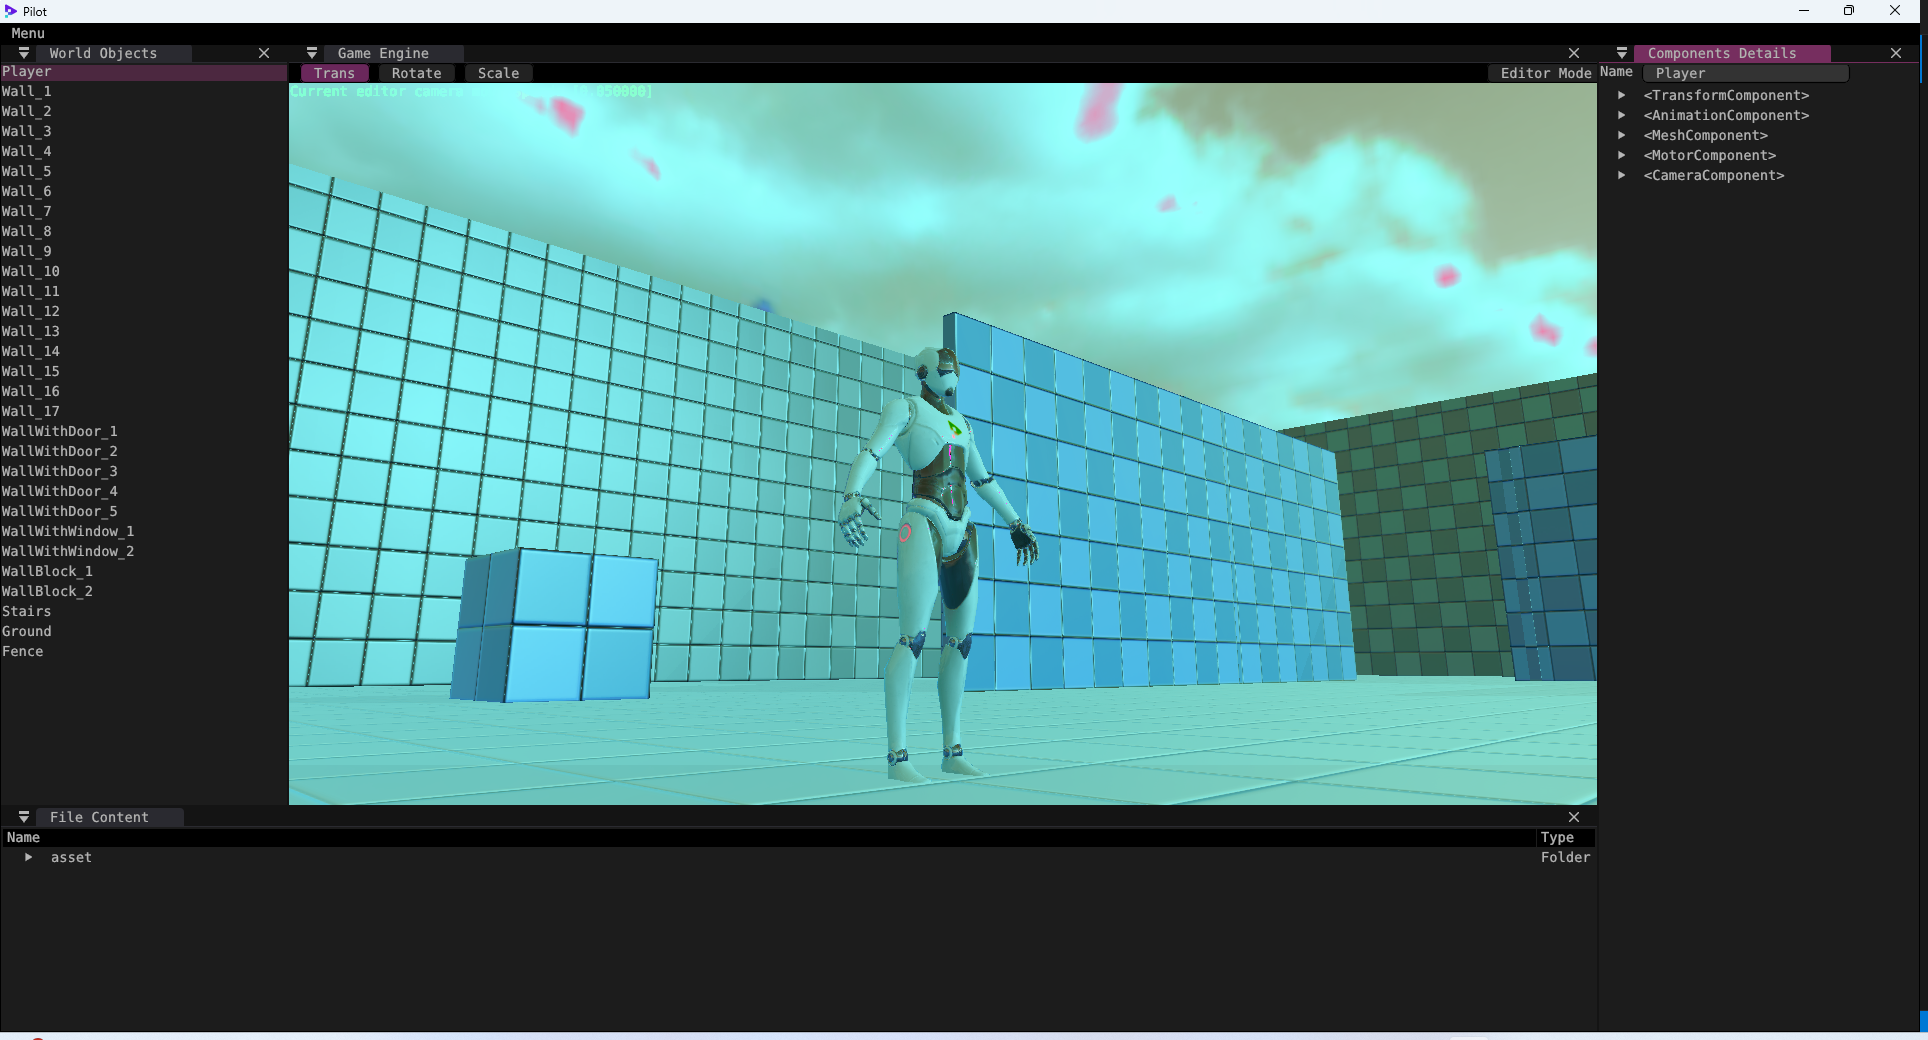
\includegraphics[width=\textwidth]{screen_shot_cube_strip_2d_64_avatar.png}
    		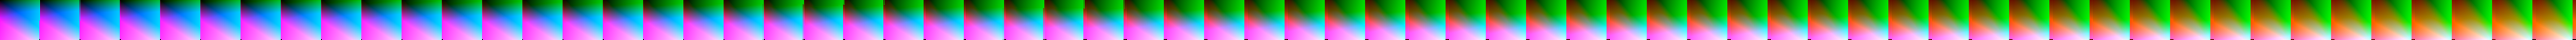
\includegraphics[width=\textwidth]{cube_strip_2d_64_avatar.png}
    		\caption{strip \& 64}
    	\end{subfigure}
    	\begin{subfigure}{0.3\textwidth}
    		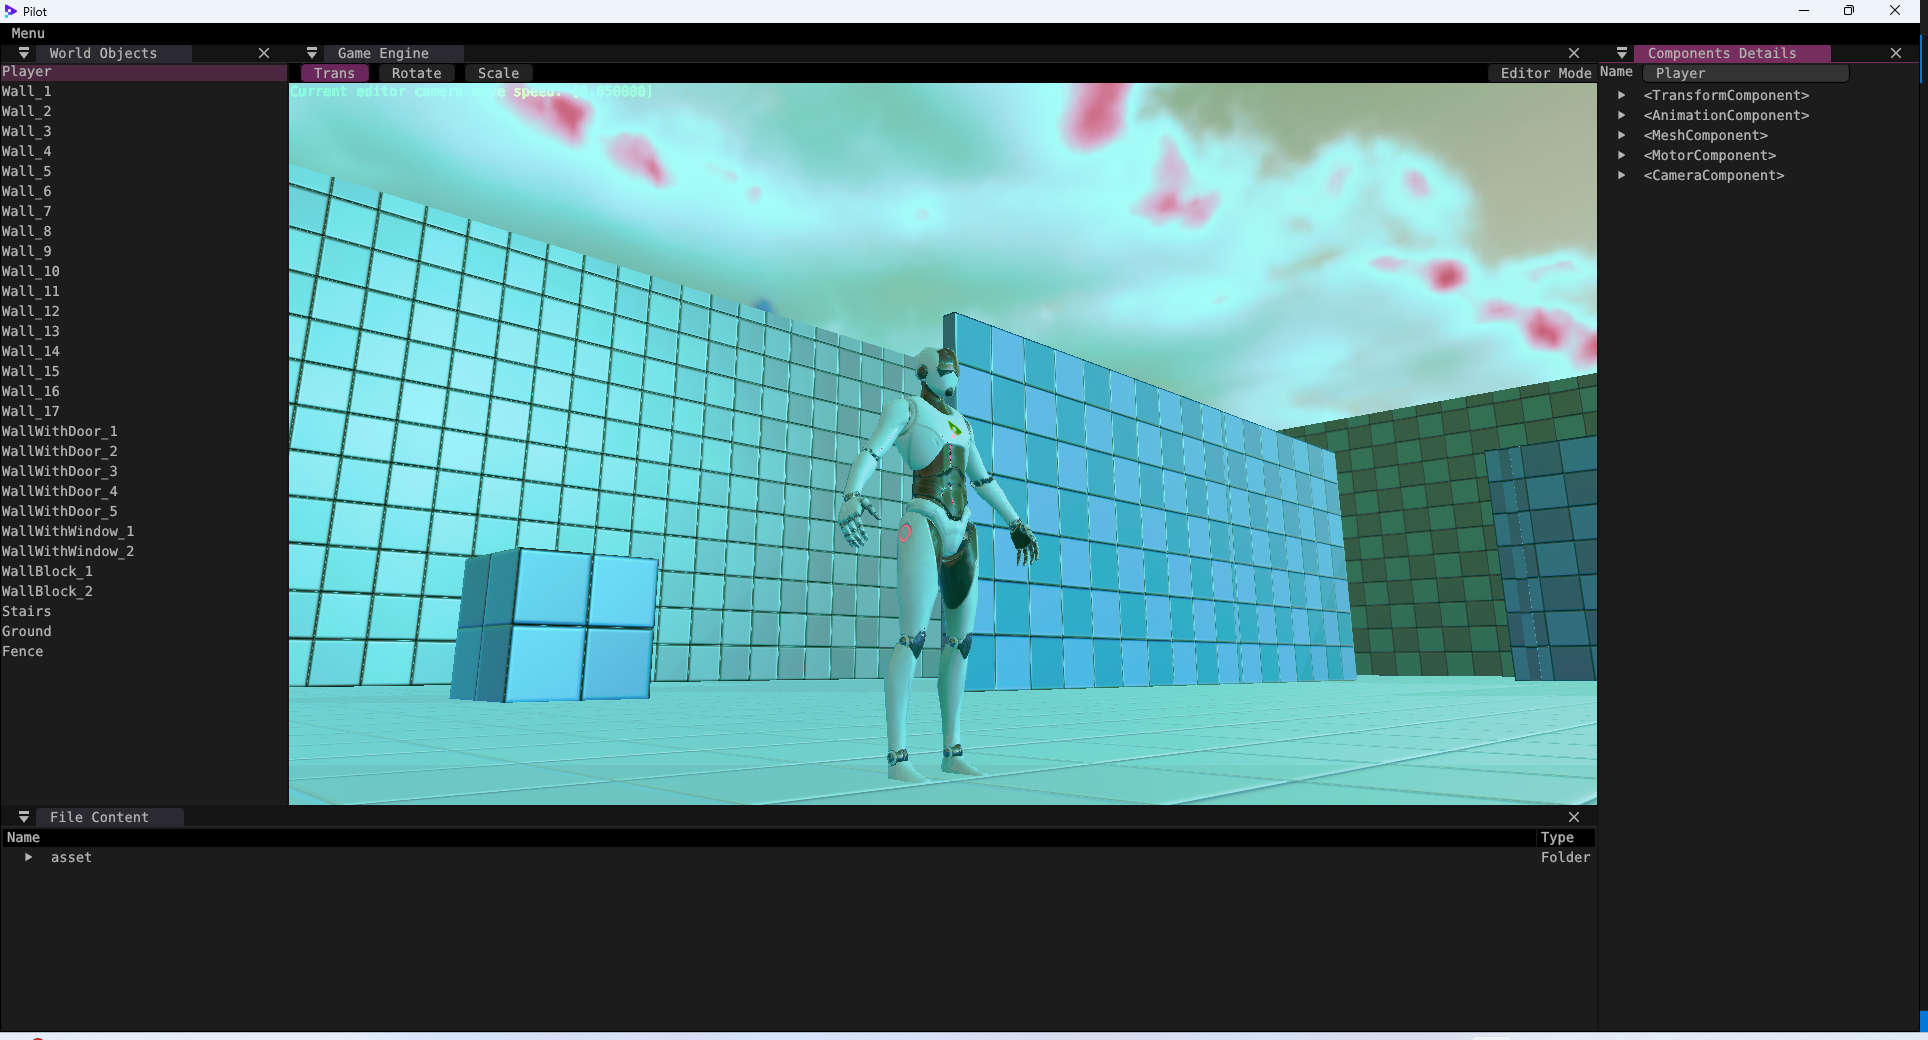
\includegraphics[width=\textwidth]{screen_shot_cube_grid_2d_16_avatar.png}
    		\caption{grid \& 16}
    	\end{subfigure}
    	\begin{subfigure}{0.3\textwidth}
    		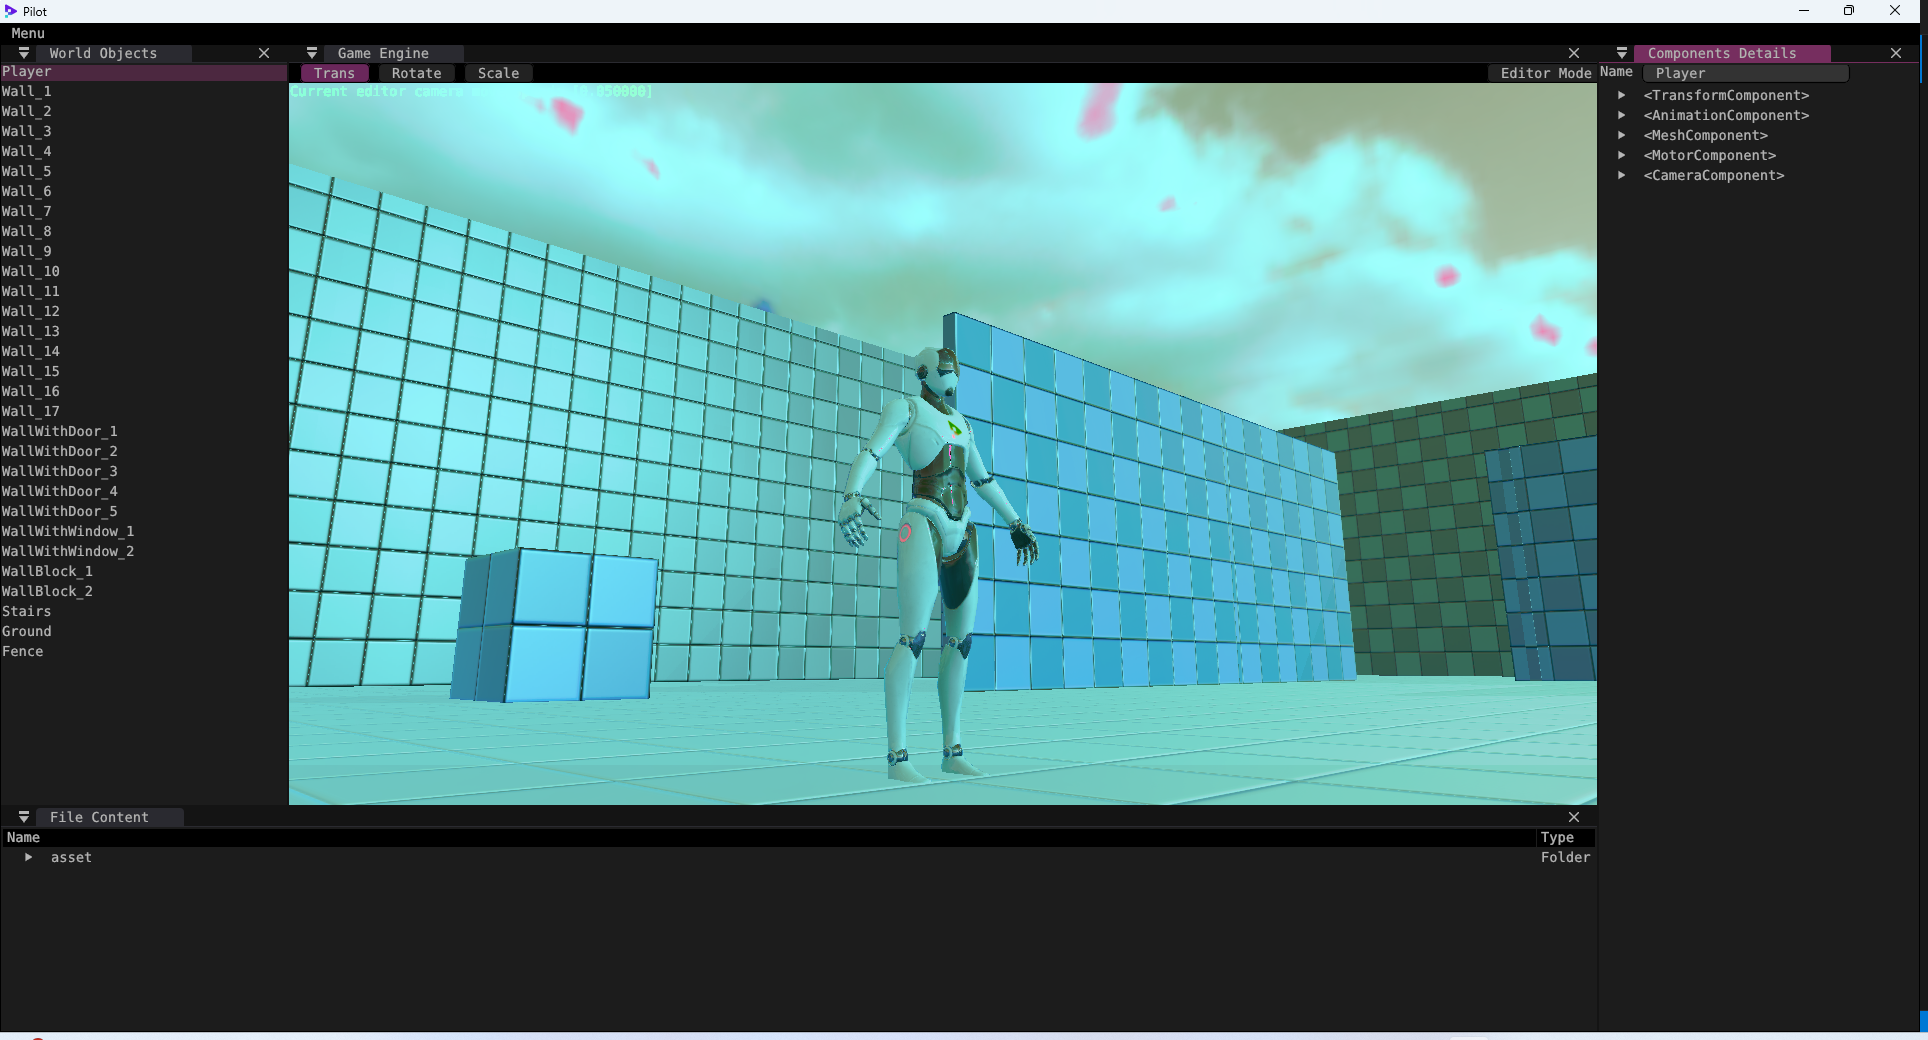
\includegraphics[width=\textwidth]{screen_shot_cube_grid_2d_32_avatar.png}
    		\caption{grid \& 32}
    	\end{subfigure}
    	\begin{subfigure}{0.3\textwidth}
    		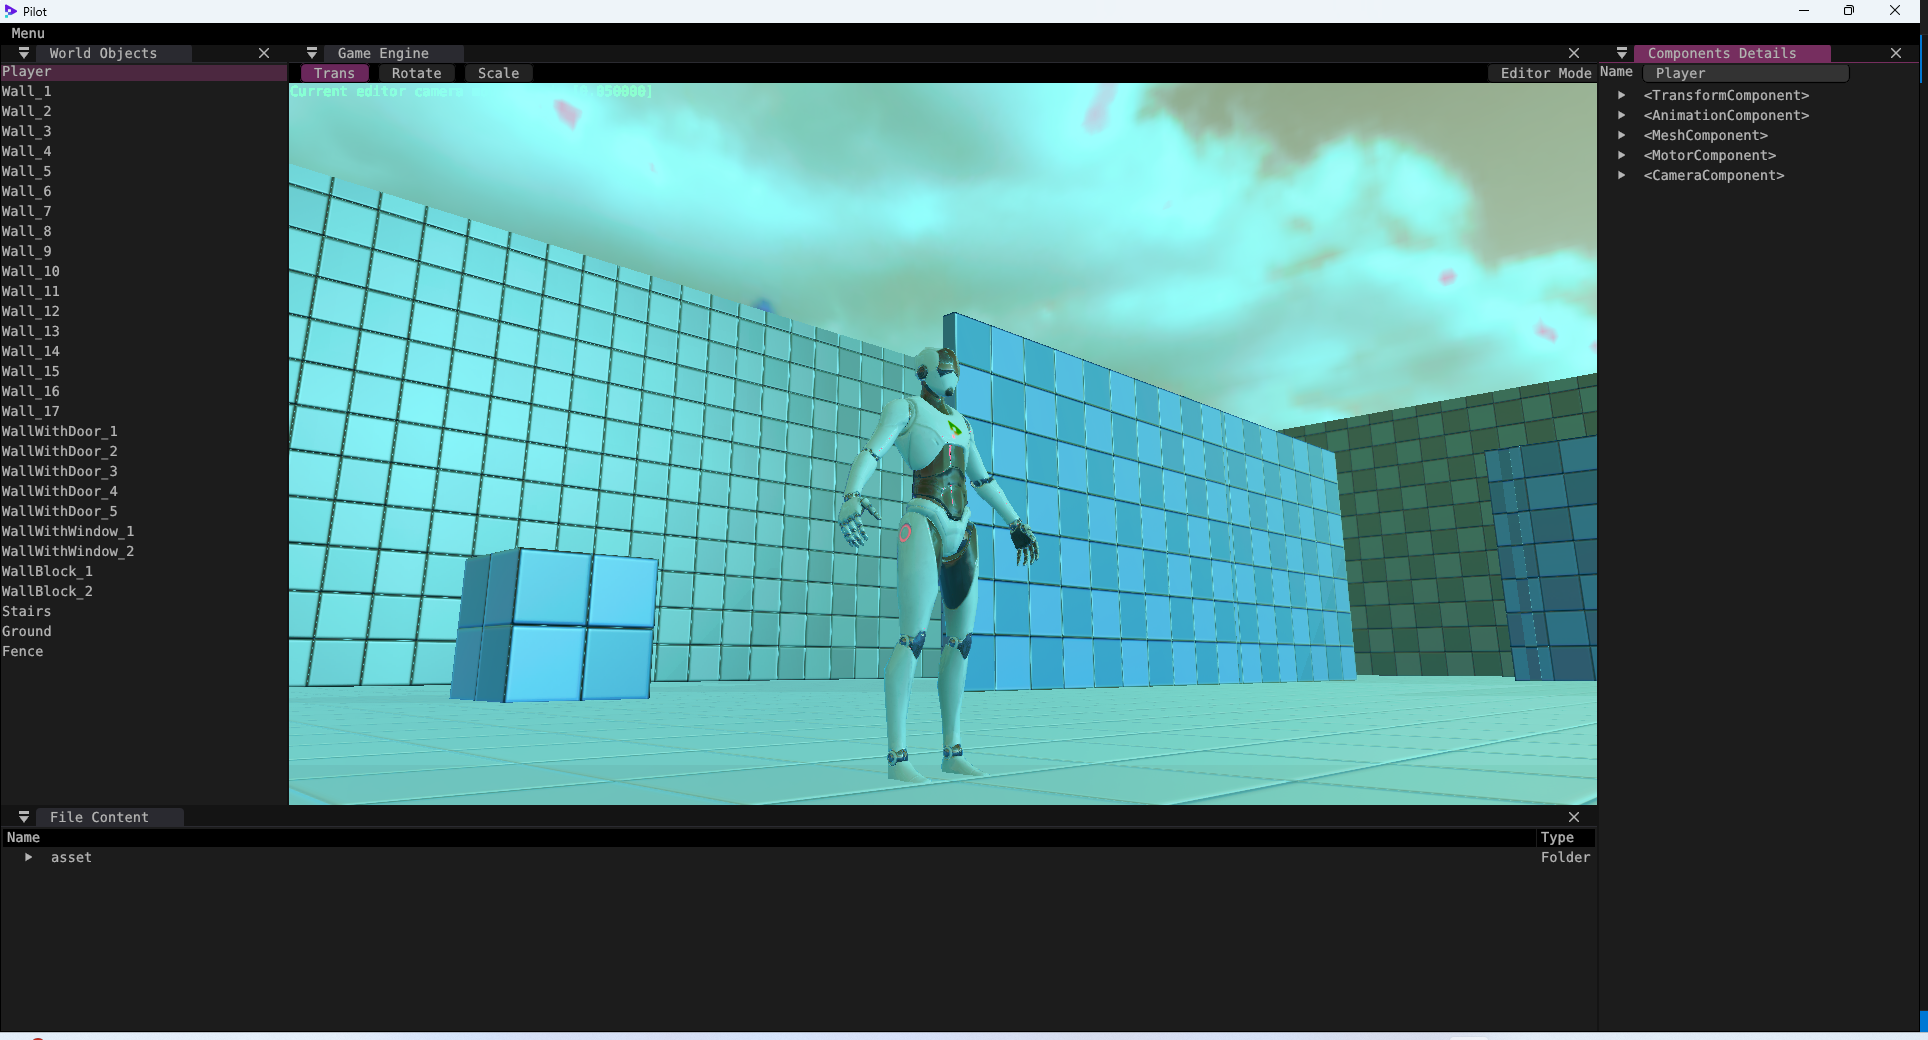
\includegraphics[width=\textwidth]{screen_shot_cube_grid_2d_64_avatar.png}
    		\caption{grid \& 64}
    	\end{subfigure} 
    	\caption{3D LUT 导出格式和大小对比图}
    \end{figure}    
    \section{基础:个性化LUT} \label{section:basic2}
    网络上分享的\textbf{3D LUTs}一般是\textbf{.cube}后缀的文件,通过免费在线3D LUT转换服务\href{https://www.color.io/free-online-lut-converter}{Visualize \& Convert 3D LUTs},可以将\textbf{.cube}文件转换成\textbf{LUT PNG Texture},主要包括\textbf{Cube Strip 2D}和\textbf{Cube Grid 3D},支持的大小包括$ 16^3 $,$ 32^3 $和$ 64^3 $。    
    \begin{figure}[!htb]
        \centering
        \begin{subfigure}{1.0\textwidth}
            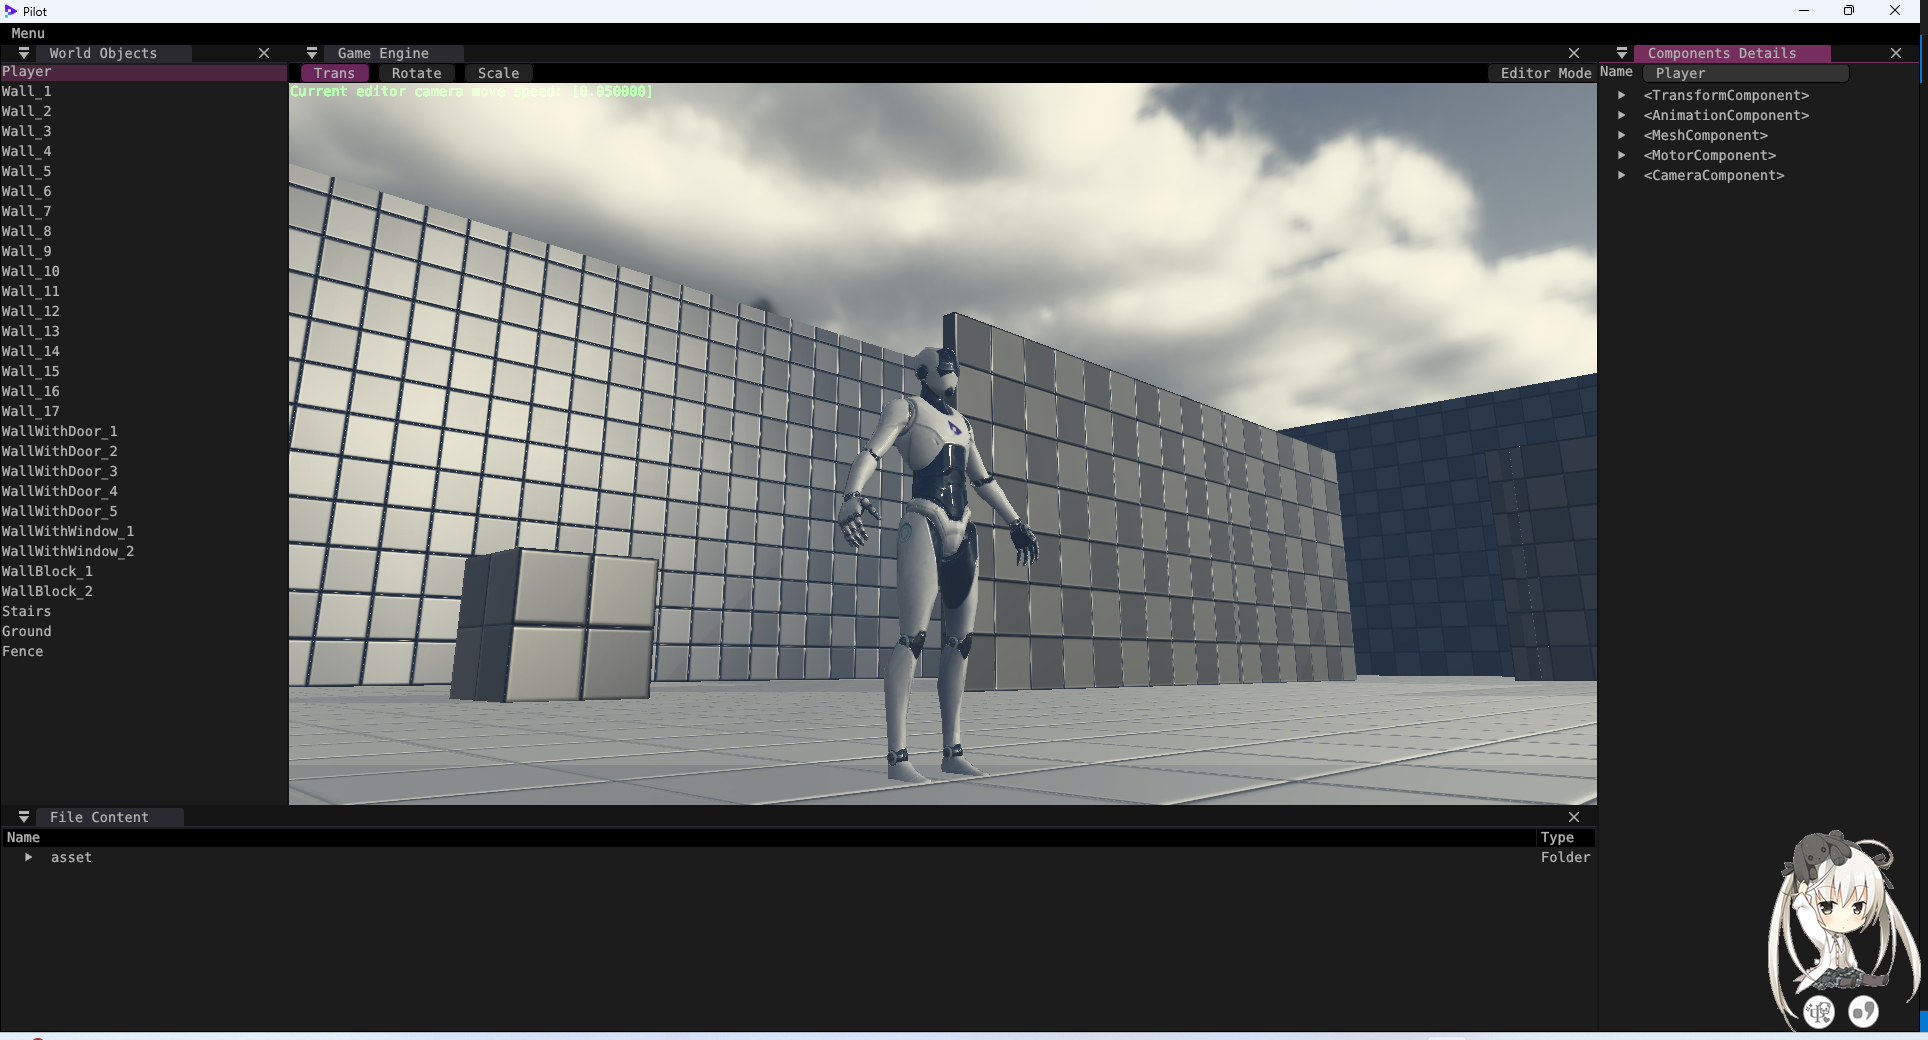
\includegraphics[width=\textwidth]{screen_shot_color_grading_map_color_grading_lut_01.png}
        \end{subfigure}
        \begin{subfigure}{1.0\textwidth}
            
\includegraphics[width=\textwidth]{color_grading_lut_01.png}
        \end{subfigure}      
        \caption{颜色分级效果截图color\_grading\_lut\_01.png}
    \end{figure}
    \begin{figure}[!htb]
        \centering
        \begin{subfigure}{1.0\textwidth}
            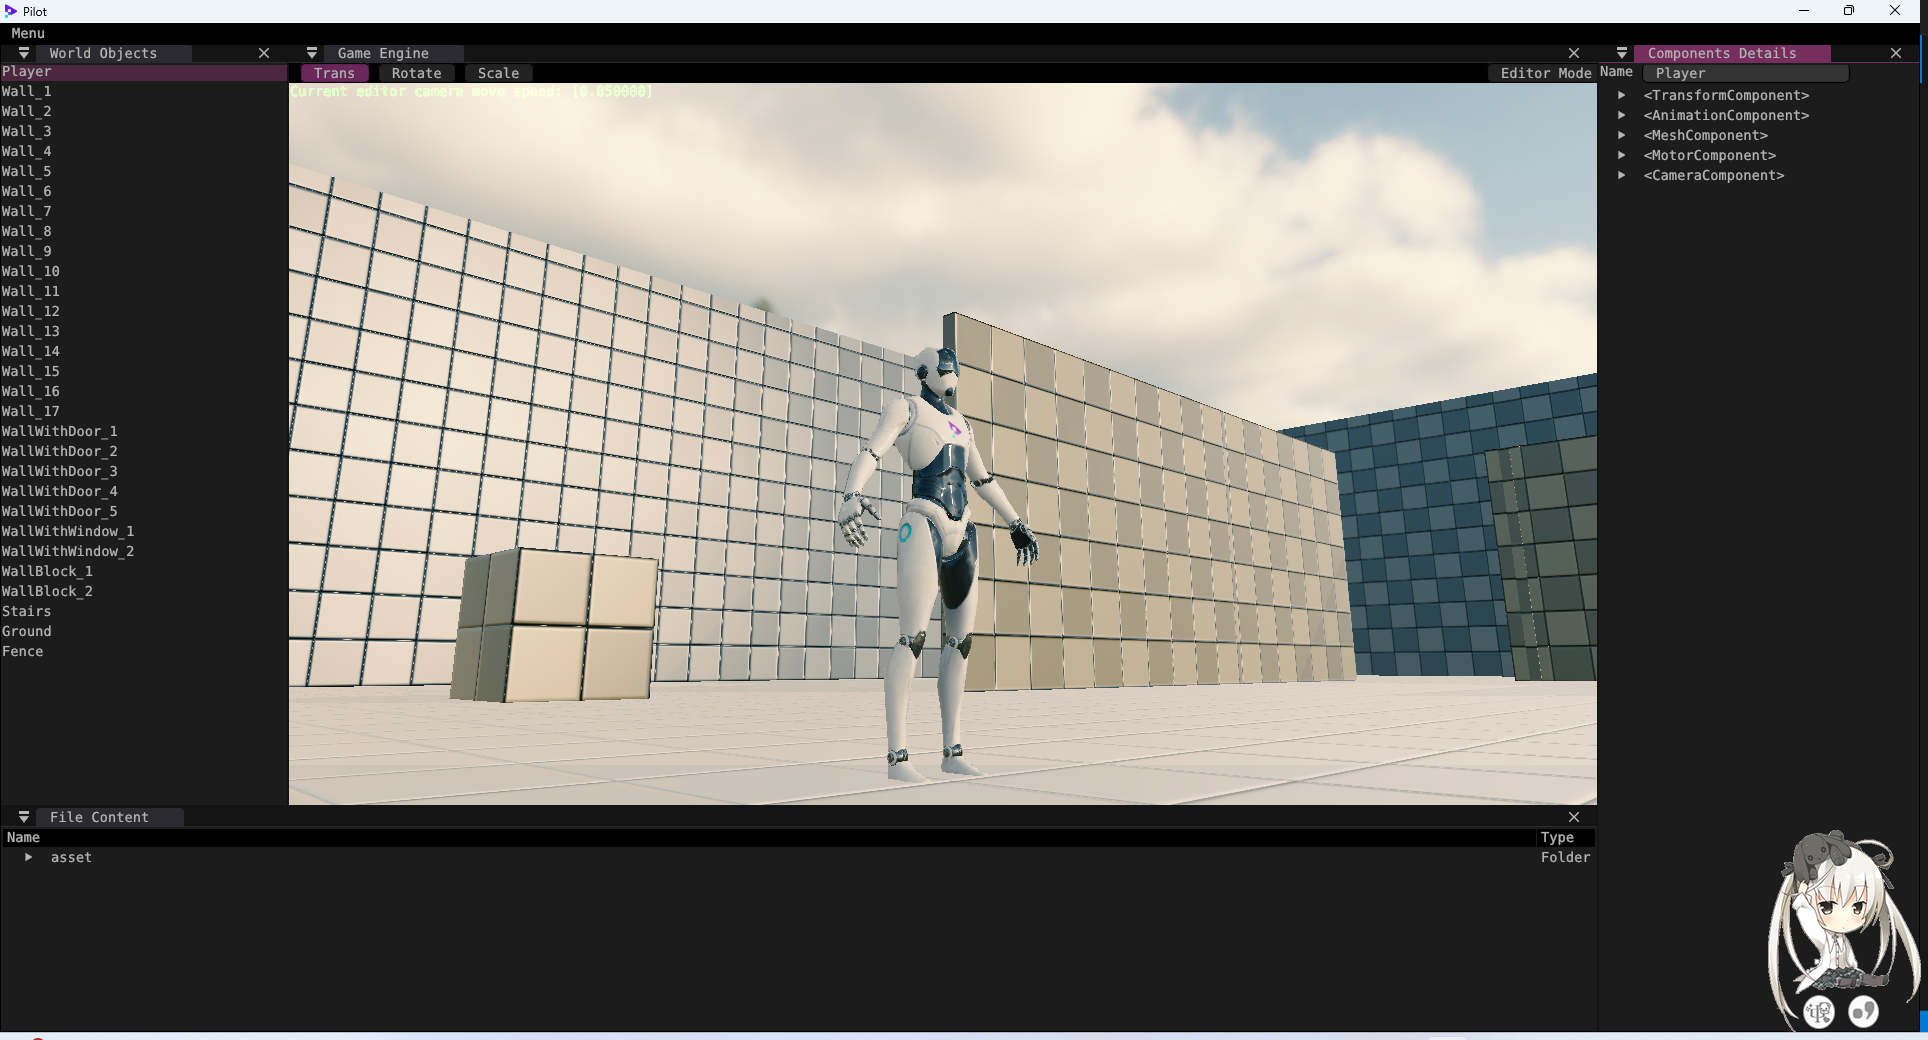
\includegraphics[width=\textwidth]{screen_shot_color_grading_map_color_grading_lut_02.png}
        \end{subfigure}
        \begin{subfigure}{1.0\textwidth}
            
\includegraphics[width=\textwidth]{color_grading_lut_02.png}
        \end{subfigure}      
        \caption{颜色分级效果截图color\_grading\_lut\_02.png}
    \end{figure}  
    \begin{figure}[!htb]
        \centering
        \begin{subfigure}{1.0\textwidth}
            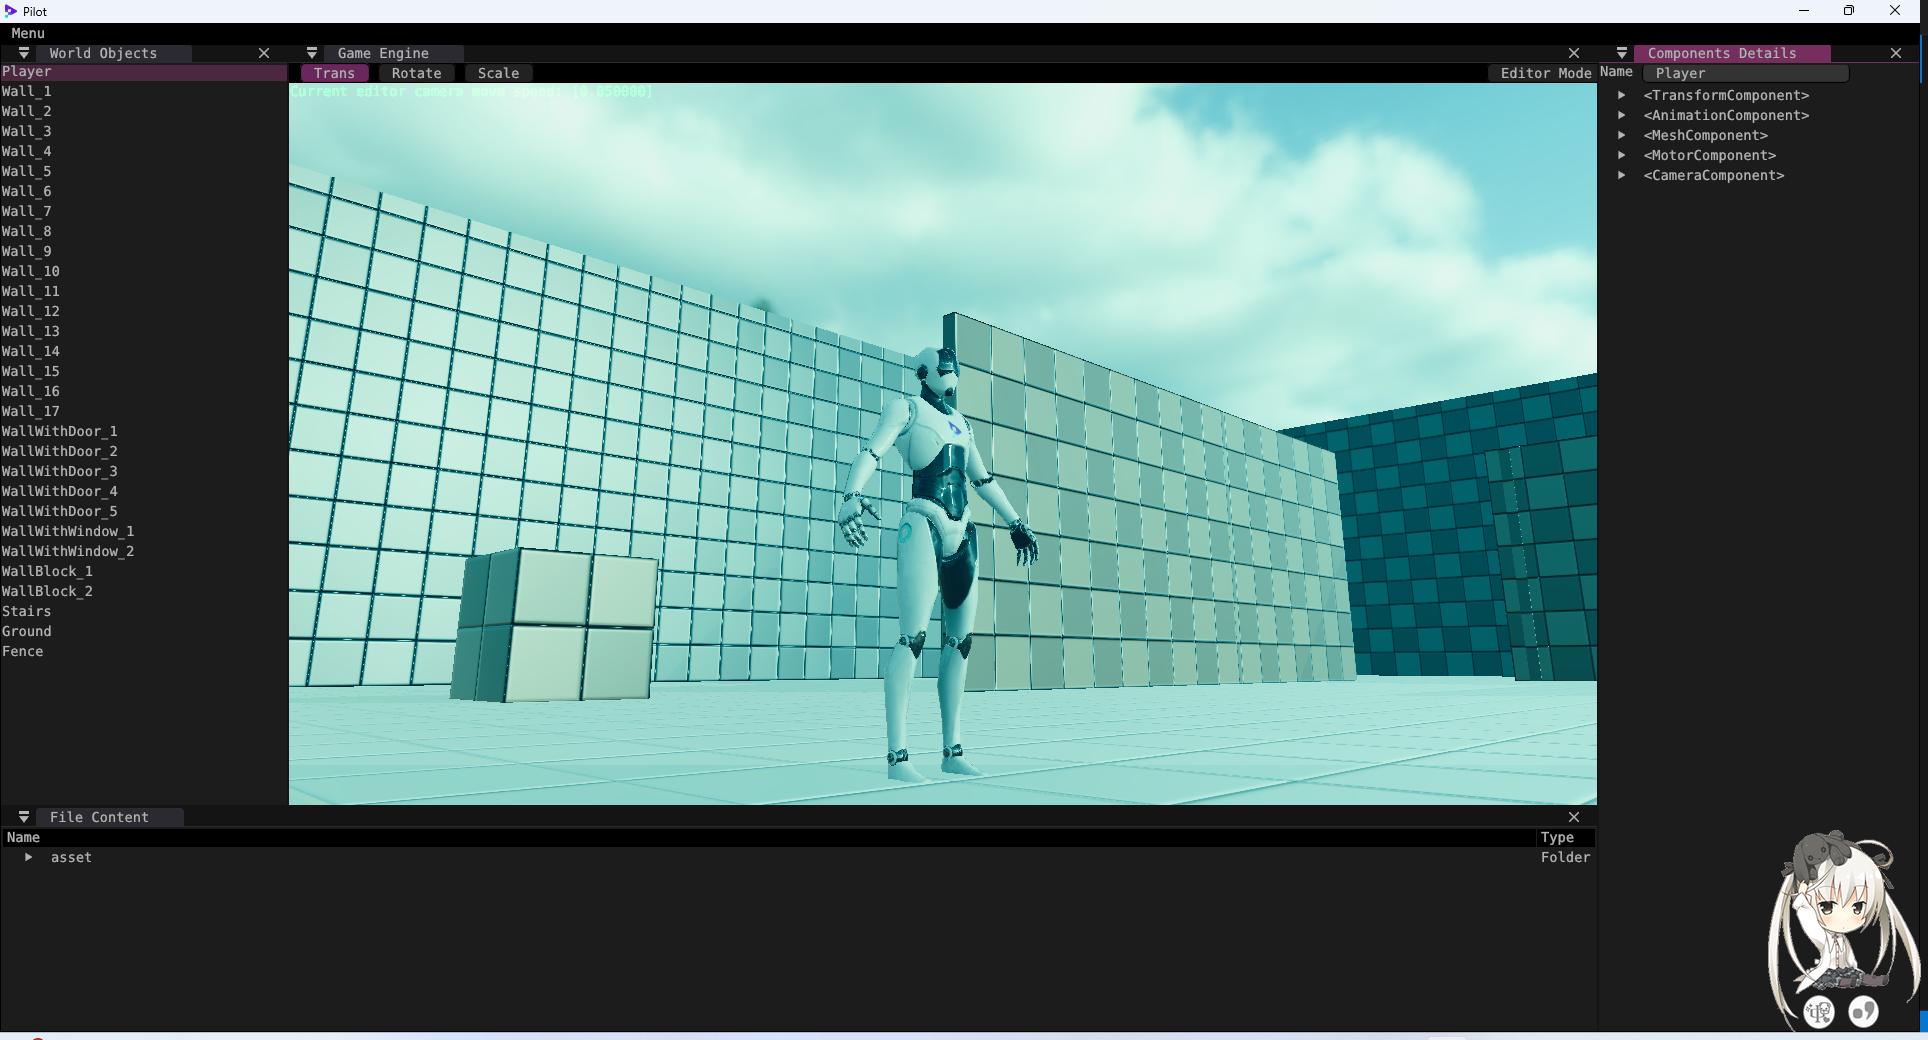
\includegraphics[width=\textwidth]{screen_shot_color_grading_map_color_grading_lut_03.png}
        \end{subfigure}
        \begin{subfigure}{1.0\textwidth}
            
\includegraphics[width=\textwidth]{color_grading_lut_03.png}
        \end{subfigure}      
        \caption{颜色分级效果截图color\_grading\_lut\_03.png}
    \end{figure}    
    \begin{figure}[!htb]
        \centering
        \begin{subfigure}{1.0\textwidth}
            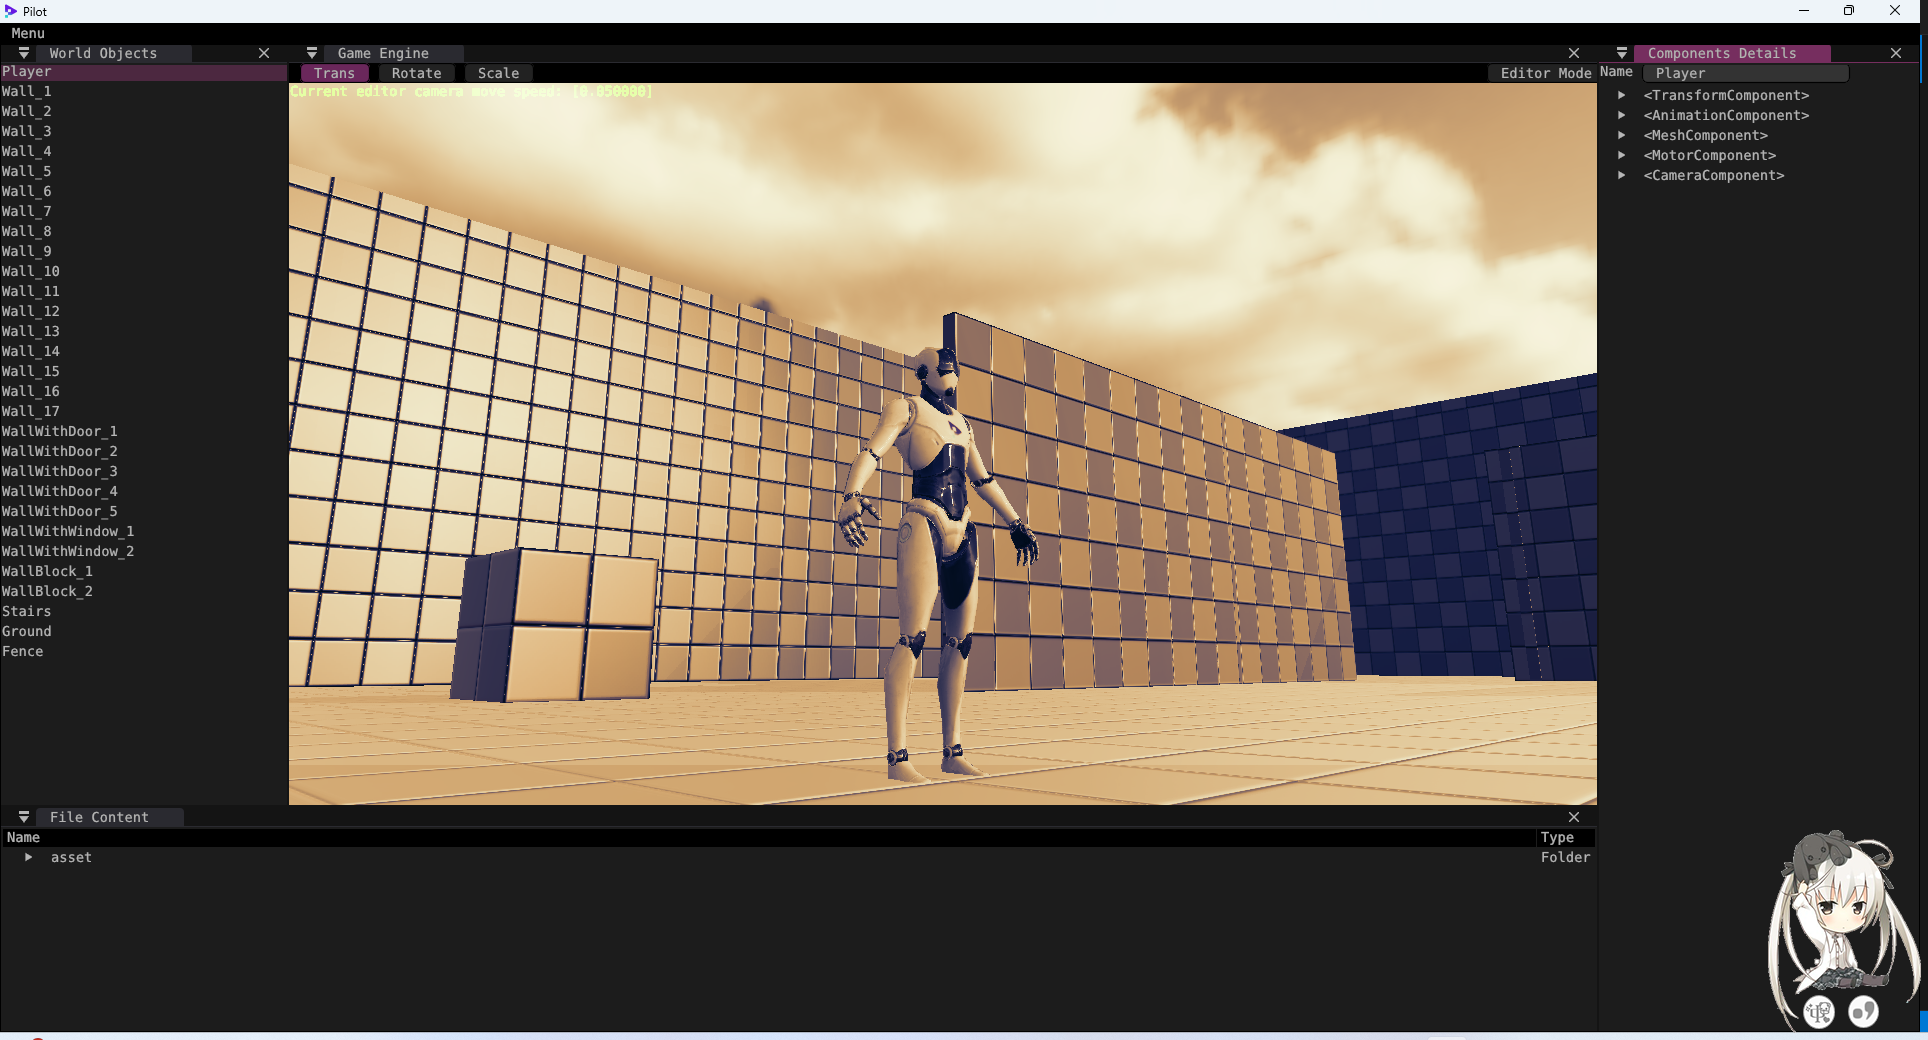
\includegraphics[width=\textwidth]{screen_shot_color_grading_map_color_grading_lut_04.png}
        \end{subfigure}
        \begin{subfigure}{1.0\textwidth}
            
\includegraphics[width=\textwidth]{color_grading_lut_04.png}
        \end{subfigure}      
        \caption{颜色分级效果截图color\_grading\_lut\_04.png}
    \end{figure}  
    \begin{figure}[htbp]
        \centering
        \begin{subfigure}{1.0\textwidth}
            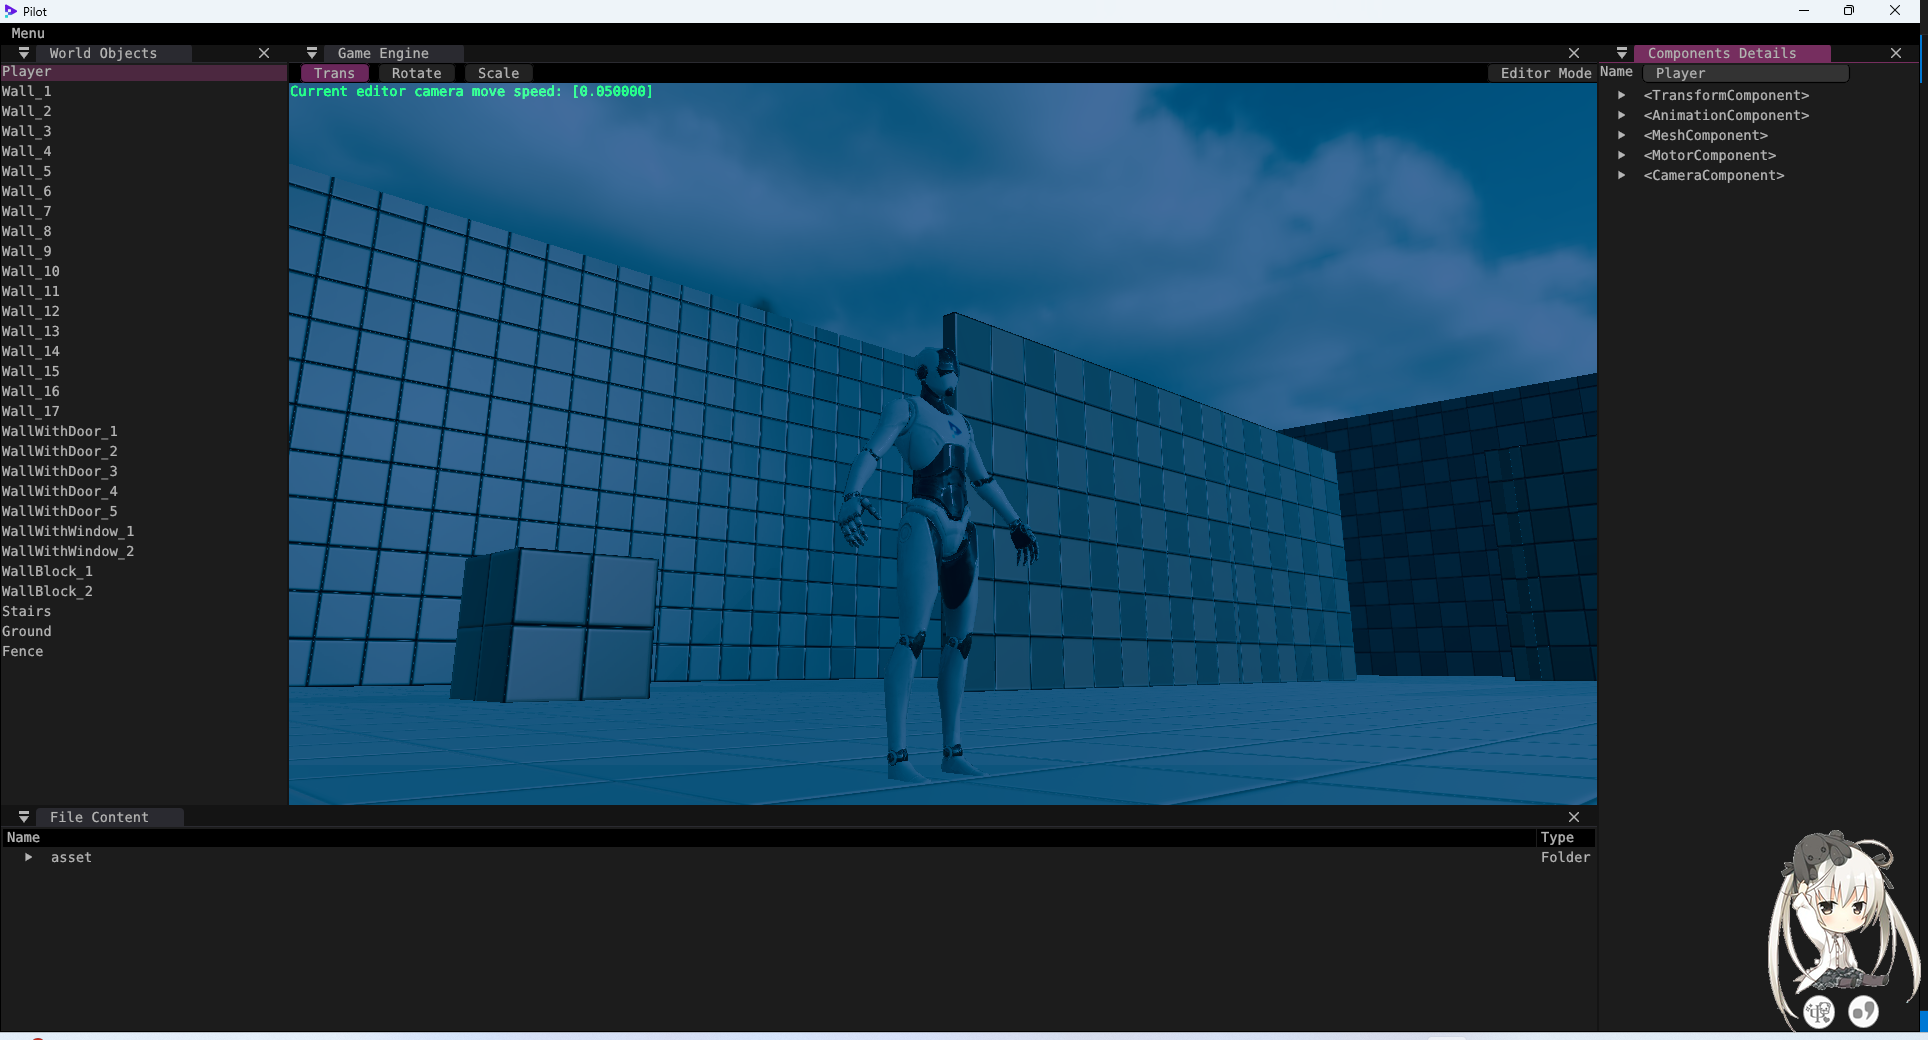
\includegraphics[width=\textwidth]{screen_shot_color_grading_map_color_grading_lut_05.png}
        \end{subfigure}
        \begin{subfigure}{1.0\textwidth}
            
\includegraphics[width=\textwidth]{color_grading_lut_05.png}
        \end{subfigure}
        \caption{颜色分级效果截图color\_grading\_lut\_05.png}
    \end{figure}    
    \begin{figure}[!htb]
        \centering
        \begin{subfigure}{1.0\textwidth}
            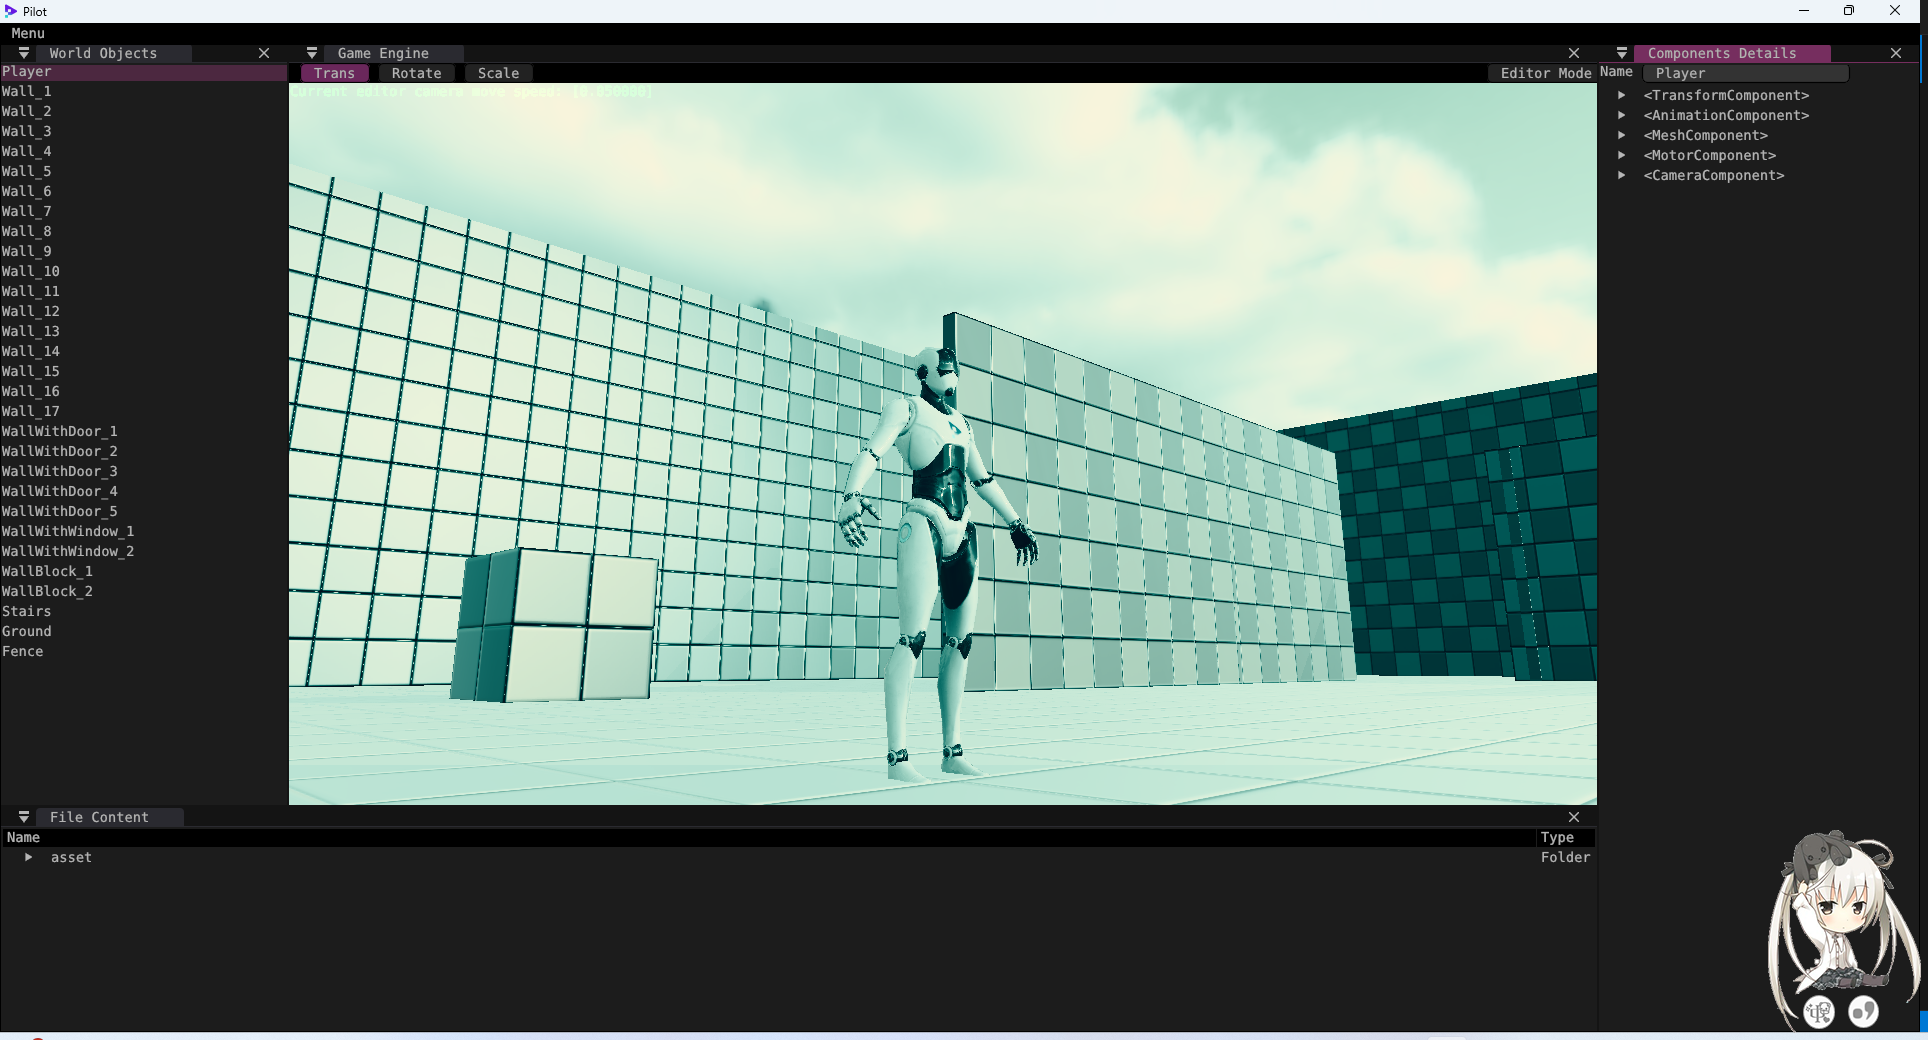
\includegraphics[width=\textwidth]{screen_shot_color_grading_map_color_grading_lut_06.png}
        \end{subfigure}
        \begin{subfigure}{1.0\textwidth}
            
\includegraphics[width=\textwidth]{color_grading_lut_06.png}
        \end{subfigure}      
        \caption{颜色分级效果截图color\_grading\_lut\_06.png}
    \end{figure}
    \begin{figure}[!htb]
    	\centering
    	\begin{subfigure}{1.0\textwidth}
    		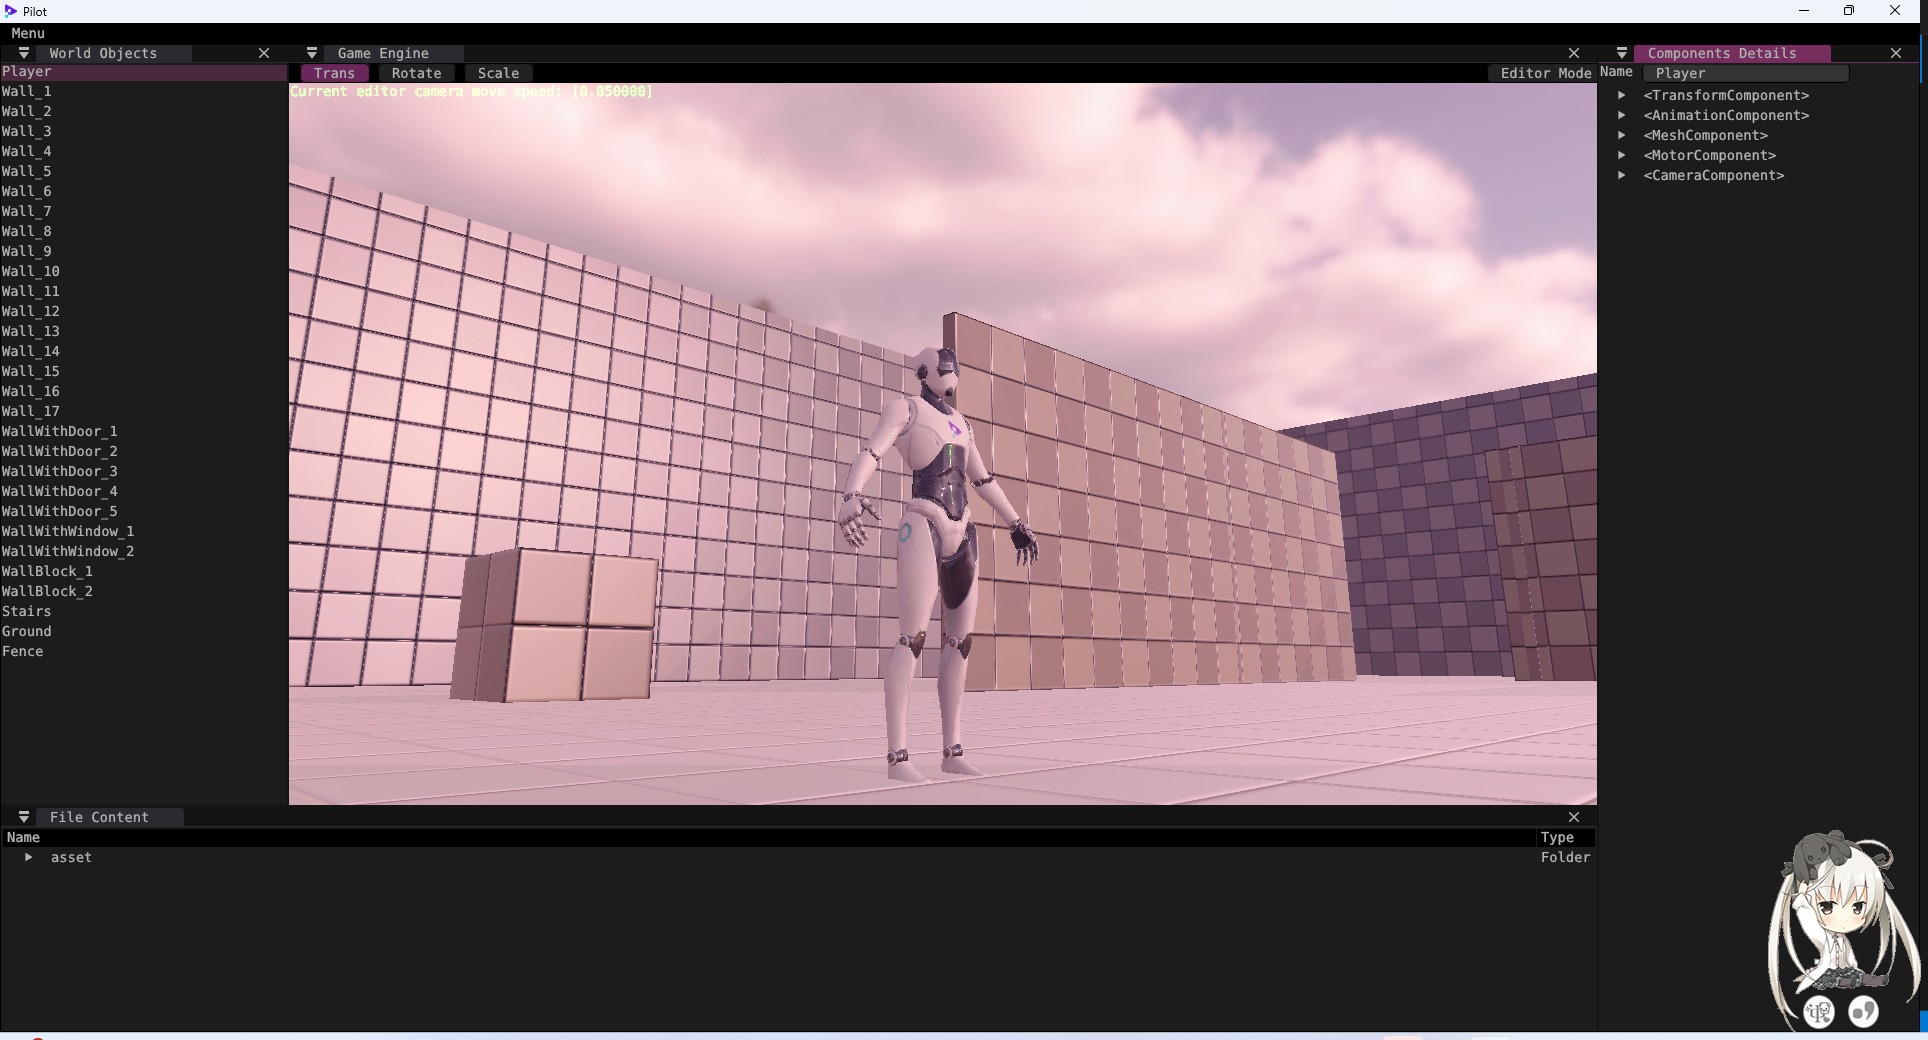
\includegraphics[width=\textwidth]{screen_shot_color_grading_LUT.png}
    	\end{subfigure}
    	\begin{subfigure}{1.0\textwidth}
    		
\includegraphics[width=\textwidth]{color_grading_LUT.jpg}
    	\end{subfigure}      
    	\caption{颜色分级效果截图color\_grading\_LUT.jpg}
    \end{figure}   
    
    \section{提高:后期处理}
    \subsection{代码实现}
    \subsubsection{vulkan\_passes.h}
    在该文件中定义后期处理效果泛光类
    \begin{minted}{c++}
class PBloomPass : public PRenderPassBase
{
public:
    void initialize(VkRenderPass render_pass, VkImageView input_attachment);
    void draw();
    void updateAfterFramebufferRecreate(VkImageView input_attachment);
private:
    void setupDescriptorSetLayout();
    void setupPipelines();
    void setupDescriptorSet();
};
    \end{minted}
    
    在枚举中添加泛光特效索引\verb|_main_camera_subpass_bloom|,\verb|_main_camera_subpass_count|枚举值为当前后期处理特效个数,
    \begin{minted}{c++}
enum
{
    _main_camera_subpass_basepass = 0,
    _main_camera_subpass_deferred_lighting,
    _main_camera_subpass_forward_lighting,
    _main_camera_subpass_bloom,
    _main_camera_subpass_tone_mapping,
    _main_camera_subpass_color_grading,
    _main_camera_subpass_ui,
    _main_camera_subpass_combine_ui,
    _main_camera_subpass_count
};
    \end{minted}    
    \subsubsection{vulkan\_manager.h}
    在该文件\verb|PVulkanManager|类的\verb|private|中定义后期处理效果泛光类成员变量
    \begin{minted}{c++}
PBloomPass m_bloom_pass;
    \end{minted}
    \subsubsection{render\_passes.cpp}
    在该文件\verb|Pilot::PVulkanManager::initializeRenderPass()|函数中调用\verb|m_bloom_pass|的\verb|initialize|方法,这里需要注意第二个参数的填写,以及根据新插入Pass的位置调整已存在的Pass初始化参数
    \begin{minted}{c++}
m_bloom_pass.initialize(
    m_main_camera_pass.getRenderPass(),
    m_main_camera_pass.getFramebufferImageViews()[_main_camera_pass_backup_buffer_odd]
);
    \end{minted}
    \subsubsection{main\_camera.cpp}
    在该文件\verb|PMainCameraPass::setupRenderPass()|函数中添加新的\verb|VkSubpassDescription|对象和\verb|VkSubpassDependency|对象
    \begin{minted}{c++}
VkAttachmentReference bloom_pass_input_attachment_reference {};
bloom_pass_input_attachment_reference.attachment = 
    &backup_odd_color_attachment_description - attachments;
bloom_pass_input_attachment_reference.layout     = VK_IMAGE_LAYOUT_SHADER_READ_ONLY_OPTIMAL;

VkAttachmentReference bloom_pass_color_attachment_reference {};
bloom_pass_color_attachment_reference.attachment = 
    &backup_even_color_attachment_description - attachments;
bloom_pass_color_attachment_reference.layout     = VK_IMAGE_LAYOUT_COLOR_ATTACHMENT_OPTIMAL;

VkSubpassDescription& bloom_pass   = subpasses[_main_camera_subpass_bloom];
bloom_pass.pipelineBindPoint       = VK_PIPELINE_BIND_POINT_GRAPHICS;
bloom_pass.inputAttachmentCount    = 1;
bloom_pass.pInputAttachments       = &bloom_pass_input_attachment_reference;
bloom_pass.colorAttachmentCount    = 1;
bloom_pass.pColorAttachments       = &bloom_pass_color_attachment_reference;
bloom_pass.pDepthStencilAttachment = NULL;
bloom_pass.preserveAttachmentCount = 0;
bloom_pass.pPreserveAttachments    = NULL;
    \end{minted}
    \begin{minted}{c++}
VkSubpassDependency dependencies[_main_camera_subpass_count] = {};
    \end{minted}
    这里需要考虑Bloom处理顺序,参考帖子\href{https://zhuanlan.zhihu.com/p/118557378}{Unity PostProcess简要分析与总结},将其置于Tone Mapping和Color Grading之前,
    \begin{minted}{c++}
dependencies_counter++;
VkSubpassDependency& bloom_pass_depend_on_deferred_lighting_pass = 
    dependencies[dependencies_counter];
bloom_pass_depend_on_deferred_lighting_pass.srcSubpass           = 
    _main_camera_subpass_deferred_lighting;
bloom_pass_depend_on_deferred_lighting_pass.dstSubpass           = 
    _main_camera_subpass_bloom;
bloom_pass_depend_on_deferred_lighting_pass.srcStageMask = 
    VK_PIPELINE_STAGE_FRAGMENT_SHADER_BIT | VK_PIPELINE_STAGE_COLOR_ATTACHMENT_OUTPUT_BIT;
bloom_pass_depend_on_deferred_lighting_pass.dstStageMask =
    VK_PIPELINE_STAGE_FRAGMENT_SHADER_BIT | VK_PIPELINE_STAGE_COLOR_ATTACHMENT_OUTPUT_BIT;
bloom_pass_depend_on_deferred_lighting_pass.srcAccessMask =
    VK_ACCESS_SHADER_WRITE_BIT | VK_ACCESS_COLOR_ATTACHMENT_WRITE_BIT;
bloom_pass_depend_on_deferred_lighting_pass.dstAccessMask =
    VK_ACCESS_SHADER_READ_BIT | VK_ACCESS_COLOR_ATTACHMENT_READ_BIT;
bloom_pass_depend_on_deferred_lighting_pass.dependencyFlags = VK_DEPENDENCY_BY_REGION_BIT;
    \end{minted}
    \verb|PMainCameraPass::draw()|函数中调用\verb|m_bloom_pass|的\verb|draw|方法,这里需要增加函数的输入参数
    \begin{minted}{c++}
bloom_pass.draw();
m_p_vulkan_context->_vkCmdNextSubpass(
    m_command_info._current_command_buffer, 
    VK_SUBPASS_CONTENTS_INLINE
);
    \end{minted}
    \subsubsection{swapchain.cpp}
    在该文件\verb|recreateSwapChain()|函数中调用\verb|m_bloom_pass|的\verb|updateAfterFramebufferRecreate|方法,这里同样需要注意第二个参数的填写,以及根据新插入Pass的位置调整已存在的Pass初始化参数
    \begin{minted}{c++}
m_bloom_pass.updateAfterFramebufferRecreate(
    m_main_camera_pass.getFramebufferImageViews()[_main_camera_pass_backup_buffer_odd]
);
    \end{minted}
    
\end{document}